% =================================================================================
% Hier ausw�hlen, ob TUD-Design oder nicht
% =================================================================================
\newif\ifTUDdesign
\TUDdesigntrue					% TUD-Design
%\TUDdesignfalse				% F�r Rechner ohne installierte TUDdesign-Pakete
% =================================================================================


% =================================================================================
% Hier Daten f�r studentische Arbeit eingeben
% =================================================================================
\newcommand{\SADATyp}{Master Thesis}
\newcommand{\SADATitel}{Kamerabasierte Fahrbahnerkennung zur automatisierten Fahrbahnf�hrung eines Modellauto}
\newcommand{\SADAStadt}{Darmstadt}
\newcommand{\SADAAutor}{Bahri Enis Demirtel}
\newcommand{\SADABetreuer}{Dr. -Ing. Eric Lenz}
\newcommand{\SADABetreuerII}{}
\newcommand{\SADABetreuerIII}{}
\newcommand{\SADABegin}{02. May 2017}
\newcommand{\SADAAbgabe}{02. November 2017}
\newcommand{\SADASeminar}{15. November 2017}
% =================================================================================


% =================================================================================
% Auswahl des IAT-Fachgebiets (rtm / rtp)
% =================================================================================
\newif\ifrtm
\rtmtrue	% rtm
%\rtmfalse	% rtp
% =================================================================================


% =================================================================================
% Erkl�rung, dass die Arbeit ohne Hilfe Dritter etc. erstellt wurde
% =================================================================================
\def\SADAVarianteErklaerung{ETIT}		% FB 18, Elektrotechnik
%\def\SADAVarianteErklaerung{MBDA}		% FB 16, Maschinenbau, Diplomarbeit
%\def\SADAVarianteErklaerung{MBSA}		% FB 16, Maschinenbau, Studienarbeit
% =================================================================================


% =================================================================================
% Ausnahmen von der automatischen Silbentrennung
% =================================================================================
\hyphenation{Aktu-ali-sie-rung Screen-shots Pa-rallel-ro-bo-ter Zu-stands-raum-mo-del-le nach-voll-zieh-bar Pro-jekt-se-mi-nar}
% =================================================================================


% =================================================================================
% Hier NICHTS �ndern!
% =================================================================================
\ifTUDdesign
	% Ggf. Option "numbers=noenddot" einf�gen, damit "Abbildung 3.1: _" statt "Abbildung 3.1.: _" verwendet wird.
	\documentclass[11pt, twoside, colorback, accentcolor=tud2c, nopartpage, bigchapter, fleqn, english, longdoc]{tudreport}
\else
	\documentclass[11pt, a4paper, twoside, fleqn, ngerman]{scrreprt}
  % F�r Entwurf auf Rechnern ohne installierte TUDdesign-Pakete	
	\usepackage{exscale}	% Korrektur math-Zeichen
	\usepackage{eurosym}

\fi
% Dieses File dient zum einbinden wichtiger und n�tzlicher Pakete.
% Nicht alle Pakete m�ssen verwendet werden.
%
\usepackage{t1enc}			% evtl. dc-Fonts
\usepackage[T1]{fontenc}	% F�r Silbentrennung bei W�rten mit Sonderzeichen (z.B. Umlaute)
\usepackage[latin1]{inputenc}
							% Um Sonderzeichen (�, �, �, ...) direkt eingeben zu k�nnen
\usepackage[english,main=english]{babel}
							% F�r Sprachenspezifisches
							% ngerman ist schon als globale Option definiert

%\usepackage{helvet}			% Helvetica als Standard-Sans-Schriftart
\usepackage[stable]{footmisc}
\usepackage{booktabs}


\usepackage{graphicx}		% zum Einbinden von Postscript
\usepackage{psfrag}			% Beschriftung der Bilder
\usepackage[tbtags]{amsmath}		% Mehr mathematischen Formelsatz
%\usepackage{amssymb}		% Mehr mathematische Symbole
%\usepackage{amsthm}

\usepackage{float}			% F�r Parameter [H] bei Flie�objekten

\usepackage{epsfig}			% Um eps-Bilder einzubinden
\usepackage{scrhack}    % Um Warnung "float@addtolists detected" zu unterdr�cken 
\usepackage{subfig}			% F�r Unterabbildungen
\usepackage{ltxtable} 		% Vereinigt TabularX und Longtable
\usepackage{rotating}		% Zum Drehen von Objekten
\usepackage{bibgerm}		% F�r deutsche Literaturverwaltung
%\usepackage{wrapfig}		% F�r kleine Bilder am Rand
%\usepackage{floatflt}		% Alternative zu wrapfig
%\usepackage[hang]{caption}	% Damit mehrzeilige Bildunterschriften gut aussehen
\usepackage{upgreek}		% F�r nicht-kursive kleine griechischen Buchstaben

\usepackage{multirow}		% F�r mehrzeilige Felder in Tabellen

\usepackage{textcomp}		% F�r Sonderzeichen im normalen Text
							% (offensichtlich in tudreport schon eingebunden)
\usepackage[ngerman]{varioref}		% F�r vref
\usepackage{color}			% F�r farbigen Text
\usepackage{placeins}		% F�r \FloatBarrier
\usepackage{xspace}
\usepackage{icomma}			% Damit nach Dezimalkommas kein Abstand eingef�gt wird

\usepackage{cancel}			% Zum Wegstreichen von Gleichungstermen

\usepackage{array}			% F�r Zellentyp "m{}" in tabular-Umgebungen (Vertikal zentriert)

\usepackage{listings}		% Um formatierten Quellcode einzubinden
\usepackage{moreverb}		% F�r Umgebung "`verbatimtab"' (Verbatim mit Tabs)
\renewcommand{\verbatimtabsize}{4\relax}	% Standardtabweite in "`verbatimtab"'
											% ist 4 Zeichen


% Das Packet hyperref immer als letztes einbinden (nur bookmark darf danach kommen)!
%\usepackage[ps2pdf, colorlinks=false, pdfborder={0 0 0}]{hyperref}
%\usepackage[ps2pdf]{hyperref}	% F�r Verlinkungen im erzeugten pdf
\usepackage{hyperref}	% F�r Verlinkungen im erzeugten pdf
\usepackage{bookmark}









\usepackage{enumitem}


  \usepackage{algorithmicx}
    \usepackage[ruled]{algorithm}
    \usepackage{algpseudocode}
    
    
   				% verwendete Pakete einbinden
% =================================================================================
% Definitionen f�r rtm / rtp
% =================================================================================
\ifrtm
	\newcommand{\SADAProf}{Prof. Dr.-Ing. Ulrich Konigorski}
  \newcommand{\SADAinstitut}{Institut f�r Automatisierungstechnik und Mechatronik\\
                             Fachgebiet Regelungstechnik und Mechatronik\\
                             \SADAProf}
  \newcommand{\SADAwebsite}{www.rtm.tu-darmstadt.de}
  \newcommand{\SADAtel}{06151/16-25200}
  \newcommand{\SADAlogo}{
\includegraphics[width=3cm]{./common/IAT_rtm}}
\else
  \newcommand{\SADAProf}{Prof. Dr.-Ing. Dr. h.c. Rolf Isermann}
  \newcommand{\SADAinstitut}{Institut f�r Automatisierungstechnik\\
                             und Mechatronik\\
                             FG Regelungstechnik und Prozessautomatisierung\\
                             \SADAProf}
  \newcommand{\SADAwebsite}{http://www.rtm.tu-darmstadt.de/rtp.html}
  \newcommand{\SADAtel}{06151/16-25170}
  \newcommand{\SADAlogo}{
\includegraphics[width=3cm]{./common/rtplogo}}
\fi
%\institution{\SADAinstitut}
% =================================================================================		
		
		
% =================================================================================
% Definitionen f�r die Erkl�rung, dass die Arbeit ohne Hilfe Dritter etc. erstellt wurde
% =================================================================================
% Die folgende Zeile deklariert die m�glichen Varianten der Erkl�rung, dass die
% Arbeit ohne Hilfe Dritter etc. erstellt wurde.
\def\ETIT{ETIT}\def\MBSA{MBSA}\def\MBDA{MBDA}
% =================================================================================


% =================================================================================
% Definitionen aus tudreport-Vorlage
% =================================================================================
\newif\ifTUDmargin
%\TUDmargintrue		% Sehr breiter rechter Rand
\TUDmarginfalse		% Schmaler (normaler) rechter Rand

\ifTUDmargin	% ggf. breiten Rand setzen
  \geometry{marginparsep=4.2mm,marginparwidth=28.64mm}
\fi

\newlength{\longtablewidth}
\setlength{\longtablewidth}{0.7\linewidth}
\addtolength{\longtablewidth}{-\marginparsep}
\addtolength{\longtablewidth}{-\marginparwidth}
% =================================================================================


% =================================================================================
% Farbige Deckseite, graue Balken auf allen anderen Seiten
% =================================================================================
\newif\ifOnlyColorFront
\OnlyColorFronttrue	    % Balken nur auf Deckblatt farbig
% \OnlyColorFrontfalse		% alle Balken farbig
% =================================================================================


% =================================================================================
% Befehle, die in scrreprt nicht exisiteren werden hier definiert, wenn diese
% Klasse verwendet wird.
% Auch die Seitenr�nder werden angepasst, so dass es grob wie mit tudreport
% aussieht.
% =================================================================================
\ifTUDdesign
	\title{\SADATitel}
	\subtitle{\SADAAutor}
	\subsubtitle{\SADATyp\ -- \SADAAbgabe  \\Supervisor: \SADABetreuer{} \SADABetreuerII{} \SADABetreuerIII{}}
	\setinstitutionlogo[height]{common/rtm_mit_schrift}
	\geometry{left=30mm, right=20mm, top=15mm, bottom=20mm}
\else
	\title{\SADATitel}
	\subtitle{}
	\author{\SADAAutor}	% scrreprt erwartet Autor
	
	\newcommand{\subsubtitle}[1]{}
	\newcommand{\settitlepicture}[1]{}
	\newcommand{\printpicturesize}{}
	\newcommand{\institution}[1]{}
    \pagestyle{headings}

  % Diese Pakete nur extra einbinden, wenn NICHT tudreport als Basis.
	\usepackage{amssymb}
	\usepackage{geometry}
	
% \settitlepicture{}	% Bild f�r Deckblatt
% \printpicturesize
\fi
% =================================================================================


% =================================================================================
% Anpassung Absatzformat
% =================================================================================
% Der Abstand der Zeilen betr�gt das 1,25-fache des Standard-Abstands von
% LaTeX. Da technische Arbeiten viele Formeln und Bilder enthalten, werden
% Abs�tze durch einen zus�tzlichen vertikalen Zwischenraum statt durch einen
% Einzug getrennt.
\linespread{1.25}
\setlength{\parindent}{0mm}
\setlength{\parskip}{1ex}
% =================================================================================


% =================================================================================
% Texte f�r die R�ckseite des Titelblatts vorgeben
% =================================================================================
\uppertitleback{}
\lowertitleback{}
\dedication{}
% =================================================================================


% =================================================================================
% Informationen (Meta-Daten) f�r pdf
% =================================================================================
\hypersetup{
	pdftitle = {\SADATitel},
	pdfsubject = {},
	pdfauthor = {\SADAAutor},
	pdfkeywords = {},
	pdfcreator = {},
	pdfproducer = {LaTeX with hyperref},
	pdfstartview = {Fit},
	pdfpagelayout = {SinglePage}
}
% =================================================================================
					% LaTeX-Einstellungen
% Dieses File dient zum definieren n�tzlicher Befehle.
% Es soll lediglich als Beispiel dienen, wie Befehle definiert werden, und welche Befehle n�tzlich sein k�nnen
%


% Inhalt
% ======
%	Allgemeine Abk�rzungen
%	Makros f�r Referenzen (Abbildungen, Zitate, ...)
%	Makros f�r Abbildungen
%	Makros f�r Einheiten, Exponenten
%	Makros f�r Formeln
%	Makros f�r Entwurf
%   Definitionen f�r Umgebungen



% Allgemeine Abk�rzungen
% ======================
	\newcommand{\bzw}{bzw.\@\xspace}
	\newcommand{\Bzw}{Bzw.\@\xspace}
	\newcommand{\bzgl}{bzgl.\@\xspace}
	\newcommand{\ca}{ca.\@\xspace}
	\newcommand{\evtl}{evtl.\@\xspace}
	\newcommand{\usw}{usw.\@\xspace}
	\newcommand{\etc}{etc.\@\xspace}
	\newcommand{\vgl}{vgl.\@\xspace}
	\newcommand{\Vgl}{Vgl.\@\xspace}
	\newcommand{\bspw}{bspw.\@\xspace}
	\newcommand{\Bspw}{Bspw.\@\xspace}
	\newcommand{\ggf}{ggf.\@\xspace}
	\newcommand{\Ggf}{Ggf.\@\xspace}



	\newcommand{\dah}{d.\thinspace{}h.\@\xspace}
	\newcommand{\Dah}{D.\thinspace{}h.\@\xspace}
	\newcommand{\iA}{i.\thinspace{}A.\@\xspace}
	\newcommand{\IA}{i.\thinspace{}A.\@\xspace}
	\newcommand{\ua}{u.\thinspace{}a.\@\xspace}
	\newcommand{\Ua}{U.\thinspace{}a.\@\xspace}
	\newcommand{\uU}{u.\thinspace{}U.\@\xspace}
	\newcommand{\UU}{u.\thinspace{}U.\@\xspace}
	\newcommand{\zB}{z.\thinspace{}B.\@\xspace}
	\newcommand{\ZB}{Zum Beispiel\xspace}
	\newcommand{\zT}{z.\thinspace{}T.\@\xspace}
	\newcommand{\ZT}{Z.\thinspace{}T.\@\xspace}



% Makros f�r Referenzen (Abbildungen, Zitate, ...)
% ================================================

	% Referenzierung auf Abbildungen, Tabellen, etc. (Hyperref-f�hig)
	\newcommand{\figref}[1]{\hyperref[#1]{\figurename\ \ref*{#1}}}
	\newcommand{\tabref}[1]{\hyperref[#1]{\tablename\ \ref*{#1}}}
	\newcommand{\equref}[1]{\hyperref[#1]{Gl.~(\ref*{#1})}}
	\newcommand{\defref}[1]{\hyperref[#1]{Definition~\ref*{#1}}}
	\newcommand{\figvref}[1]{\hyperref[#1]{\figurename}\vref{#1}}
	\newcommand{\tabvref}[1]{\hyperref[#1]{\tablename}\vref{#1}}
	\newcommand{\equvref}[1]{\hyperref[#1]{Gl.~(\ref*{#1}) auf Seite \pageref*{#1}}}
	\newcommand{\pagerefh}[1]{\hyperref[#1]{Seite~\pageref*{#1}}}
	\newcommand{\secref}[1]{\hyperref[#1]{Abschnitt~\ref*{#1}}}
	\newcommand{\charef}[1]{\hyperref[#1]{Kapitel~\ref*{#1}}}
	\newcommand{\lstref}[1]{\hyperref[#1]{Listing~\ref*{#1}}}


	% Zitate mit Seitenangabe in Fu�note
%	\newcommand{\citep}[2]{\cite{#1}\footnote{Seite #2}}
%	\newcommand{\citepp}[2]{\cite{#1}\footnote{Seiten #2}}
	\newcommand{\citep}[2]{\cite{#1} (S. #2)}
	\newcommand{\citepp}[2]{\cite{#1} (S. #2)}
	
	
% Makros f�r Abbildungen
% ======================
	% zum Skalieren nach Ersetzen durch psfrag
	\newcommand{\incgraphicsw}[2]{\resizebox{#1}{!}{\includegraphics{#2}}}


% Textbausteine
% =============
	% Produktnamen
	\newcommand{\Matlab}{\textsc{Matlab}}
	\newcommand{\Matlabreg}{\textsc{Matlab}\textsuperscript{\tiny \textregistered}}
	\newcommand{\MatSim}{\textsc{Matlab/Simulink}}
	\newcommand{\Simulink}{\textsc{Simulink}}
	\newcommand{\Simulinkreg}{\textsc{Simulink}\textsuperscript{\tiny \textregistered}}



% Makros f�r Einheiten, Exponenten
% ================================

	\newcommand{\unit}[1] { \ensuremath{\mathrm{#1}}}
	
	% Wert mit Einheit (mit kleinem Leerzeichen dazwischen), aus Text- UND Math-Modus
	\newcommand{\valunit}[2]{\ensuremath{#1\,\mrm{#2}}}


	% "�C", im Text- oder Mathe-Modus
	\newcommand{\degC}{
		\ifmmode
			^\circ \mrm{C}%
		\else
			\textdegree C%
		\fi}

	\newcommand{\degree}{
		\ifmmode
			^\circ%
		\else
			\textdegree%
		\fi}
	
	% F�r Exponentenschreibweise ( Anwendung: 123\E{3} )
	\newcommand{\E}[1]{ \ensuremath{\cdot 10^{#1}} }
	
	\newcommand{\eexp}[1]{ \mathrm{e}^{#1} }
	\newcommand{\iu}{ \mathrm{j} }

	\newcommand{\todots}{ ,\,\hdots,\, }


% Makros f�r Formeln
% ==================

    \newcommand{\mat}[1]{{\ensuremath{\boldsymbol{\mathrm{#1}}}}}

	\newcommand{\AP} { \mathrm{AP} }
	\newcommand{\doti} {(i)^\cdot}

	% Definition f�r Vektor und Matizen
	\newcommand{\ve}[1]{\ensuremath{\mathbf{#1}}}
	\newcommand{\ma}[1]{\ensuremath{\mathbf{#1}}}

	% Definition f�r Vektor und Matizen
	\newcommand{\ves}[1]{\ensuremath{\boldsymbol{#1}}}
	\newcommand{\mas}[1]{\ensuremath{\boldsymbol{#1}}}
	
	
	\newcommand{\inprod}[2]{\langle #1,\,#2 \rangle}
	
	\newcommand{\ul}[1]{\underline{#1}}

	% gerades "d" (z.B. f�r Integral)
	\newcommand{\ud} { \mathrm{d} }
	
	% normaler Text in Formeln
	\newcommand{\tn}[1] { \textnormal{#1} }
	
	% nicht-kursive Schrift in Formeln
	\newcommand{\mrm}[1] { \mathrm{#1}}
	
	% gerades "T" f�r Transponiert
	\newcommand{\transp}{\mathrm{T}}
	
	% gerades "rg"
	\newcommand{\rang}[1]{\mathrm{rg}(#1)}

	% F�r geklammerte Ausdr�cke mit Index (Subscript)
	% (einmal mit kursiven Index, einmal mit geradem Index)
	\newcommand{\grpsb}[2] { \left( #1 \right)_{#2} }
	\newcommand{\grprsb}[2] { \left( #1 \right)_{\mathrm{#2}} }

	% Ableitungen und Integrale
		% "normale" Ableitung (mit geraden "d"s)
		\newcommand{\normd}[2] { \frac{\mathrm{d} #1 }{\mathrm{d} #2 } }
		\newcommand{\normdat}[3] { \left. \frac{\mathrm{d} #1 }{\mathrm{d} #2 } \right|_{#3} }
	
		% Materielle Ableitung
		\newcommand{\matd}[2] { \frac{\mathrm{D} #1 }{\mathrm{D} #2 } }
		\newcommand{\matdat}[3] { \left. \frac{\mathrm{D} #1 }{\mathrm{D} #2 } \right|_{#3} }
	
		% Partielle Ableitung
		\newcommand{\partiald}[2] { \frac{\partial #1 }{\partial #2 } }
		\newcommand{\partialdat}[3] { \left. \frac{\partial #1 }{\partial #2 } \right|_{#3} }
	
	
	% Transformationen
	\newcommand{\FT}[1] { \mathfrak{F} \left\{ #1 \right\} }
	\newcommand{\FTabs}[1]{\left| \mathfrak{F} \left\{ #1 \right\} \right|}
	\newcommand{\IFT}[1] { \mathfrak{F}^{-1} \left\{ #1 \right\} }
	\newcommand{\DFT}[1]{\mathrm{DFT} \left\{ #1 \right\}}
	\newcommand{\DFTabs}[1]{\left| \mathrm{DFT} \left\{ #1 \right\} \right|}

	\newcommand{\Laplace}[1]{\mathfrak{L}\left (#1\right)} % L-Transformation
	\newcommand{\InvLaplace}[1]{\mathfrak{L^{-1}}\left (#1\right )} % L-Transformation, invers
	\newcommand{\invtrans}{\quad\bullet\!\!-\!\!\!-\!\!\circ\quad}
	\newcommand{\trans}{\quad\circ\!\!-\!\!\!-\!\!\bullet\quad}


	\newcommand{\mlfct}[1]{{\texttt #1}}
	\newcommand{\mlvar}[1]{{\texttt #1}}


	% Manche textcomp-Zeichen funktionieren mit dem TU-Design nicht, diese k�nnen dann mit diesem
	% Befehl gesetzt werden.
	\newcommand{\textcompstdfont}[1]{{\fontfamily{cmr} \fontseries{m} \fontshape{n} \selectfont #1}}
	


% =================================================================================
% Defintionen f�r Mathe-Umgebungen
% =================================================================================
	
\newtheorem{theorem}{Satz}
\newtheorem{lemma}[theorem]{Lemma}	% Selber Z�hler wie theorem
\newtheorem{definition}{Definition}
% =================================================================================


% =================================================================================
% Defintionen f�r Beispiel-Umgebung
% =================================================================================
\newcounter{examplenumber}[chapter]      % Neuer Counter bspnummer nummeriert nach Kapitel
\def\theexamplenumber{\thechapter.\arabic{examplenumber}}

\newenvironment{example}[1][]
{\vskip 3\parskip plus 1pt minus 1pt \refstepcounter{examplenumber}
\vspace{.3cm} \begin{addmargin}[1cm]{0cm} \noindent \textbf{Beispiel \theexamplenumber}: \textbf{#1}\par}
{\end{addmargin} \par \vspace{.3cm}}

% Alternative, einfachere Beispielumgebung:
% \newtheorem{example}{Beispiel}
% =================================================================================




% =================================================================================
% Definitionen f�r Listingsumgebung
% =================================================================================

\lstloadlanguages{Matlab}

\lstdefinestyle{Matlab_colored_smallfont}
{
	language = Matlab,
	tabsize = 4,
	framesep = 3mm,
	frame=tb,
	classoffset = 0,	
	basicstyle = \footnotesize\ttfamily,
	keywordstyle = \bfseries\color[rgb]{0,0,1},
	commentstyle = \itshape\color[rgb]{0.133,0.545,0.133},
	stringstyle = \color[rgb]{0.627,0.126,0.941},
	extendedchars = true,
	breaklines = true,
	prebreak = \textrightarrow,
	postbreak = \textleftarrow,
	%escapeinside = {(*@}{@*)},
	%moredelim = [s][\itshape\color[rgb]{0.5,0.5,0.5}]{[.}{.]},
	numbers = left,
	numberstyle = \tiny,
	stepnumber = 5
}

\lstdefinestyle{Matlab_colored}
{
	language = Matlab,
	tabsize = 4,
	framesep = 3mm,
	frame=tb,
	classoffset = 0,	
	basicstyle = \ttfamily,
	keywordstyle = \bfseries\color[rgb]{0,0,1},
	commentstyle = \itshape\color[rgb]{0.133,0.545,0.133},
	stringstyle = \color[rgb]{0.627,0.126,0.941},
	extendedchars = true,
	breaklines = true,
	prebreak = \textrightarrow,
	postbreak = \textleftarrow,
	%escapeinside = {(*@}{@*)},
	%moredelim = [s][\itshape\color[rgb]{0.5,0.5,0.5}]{[.}{.]},
	numbers = left,
	numberstyle = \tiny,
	stepnumber = 5
}


\lstdefinestyle{C_colored_smallfont}
{
	language=C,
	tabsize = 4,
	framesep = 3mm,
	frame=tb,	
	classoffset = 0,	
	basicstyle = \footnotesize\ttfamily,
	keywordstyle = \bfseries\color[rgb]{0,0,1},
	commentstyle = \itshape\color[rgb]{0.133,0.545,0.133},
	stringstyle = \color[rgb]{0.627,0.126,0.941},
	extendedchars = true,
	breaklines = true,
	prebreak = \textrightarrow,
	postbreak = \textleftarrow,
	%escapeinside = {(*@}{@*)},
	%moredelim = [s][\itshape\color[rgb]{0.5,0.5,0.5}]{[.}{.]},
	numbers = left,
	numberstyle = \tiny,
	stepnumber = 5
}

\lstdefinestyle{C_colored}
{
	language=C,
	tabsize = 4,
	framesep = 3mm,
	frame=tb,
	classoffset = 0,	
	basicstyle = \ttfamily,
	keywordstyle = \bfseries\color[rgb]{0,0,1},
	commentstyle = \itshape\color[rgb]{0.133,0.545,0.133},
	stringstyle = \color[rgb]{0.627,0.126,0.941},
	extendedchars = true,
	breaklines = true,
	prebreak = \textrightarrow,
	postbreak = \textleftarrow,
	%escapeinside = {(*@}{@*)},
	%moredelim = [s][\itshape\color[rgb]{0.5,0.5,0.5}]{[.}{.]},
	numbers = left,
	numberstyle = \tiny,
	stepnumber = 5
}
		% oft verwendete Befehle
% =================================================================================


% =================================================================================
% Hier beginnt das eigentliche Dokument
% =================================================================================
\begin{document}
\selectlanguage{ngerman}
\maketitle

% Die Farbe der Identit�tsleiste wird auf Grau umgestellt, damit nicht alle Seiten
% farbig gedruckt werden m�ssen
\ifTUDdesign
	\ifOnlyColorFront	% ggf. nachfolgende Balken andere Farbe zuweisen
		\makeatletter 	% ben�tigt, um die @-Befehle auszuf�hren
    \renewcommand{\@TUD@largerulecolor}{\color{tud0b}}% am besten gleiche Farbe wie in der ersten Zeile und die Zahl durch die 0 ersetzen, dann hat das Grau die richtige Intensit�t
    \makeatother
	\fi
\fi


\pagenumbering{roman}	% Bis zum Hauptteil werden r�mische Seitenzahlen verwendet

% =================================================================================
% Spezielle Seiten f�r studentische Arbeiten
% =================================================================================
\cleardoublepage
\section*{Aufgabenstellung}
Im Rahmen des Projektseminars Echtzeitsysteme werden von Studenten The-
men aus dem Bereich des autonomen Fahrens bearbeitet. Bisher haben sich die
Fahrzeuge dabei frei im Raum bewegt, und eine Orientierung st�tzte sich im We-
sentlichen auf W�nde, die �ber Ultraschallsensoren und 2D- sowie 3D-Kameras
erkannt werden.

Um realistischere Fahrsituationen zu behandeln, soll in Zukunft auf eine Fahrt
innerhalb von markierten Fahrspuren umgestellt werden. Als mittelfristiges Ziel
ist die Teilnahme studentischer Gruppen am Carolino-Cup zu nennen. Die Spe-
zifikation der Fahrspurmarkierungen ist daher den Regeln zum Carolino-Cup zu
entnehmen.

Basisziel dieser Arbeit ist die Implementierung einer geeigneten Methode, die
anhand von Kameradaten die aktuelle Fahrspur und die Nachbarfahrspur erkennt.
Dabei ist der Verlauf der Fahrspur in einer geeigneten mathematischen Beschrei-
bung anzugeben, aus der sich die Breite der Fahrspur, deren Kr�mmung und Kr�m-
mungs�nderung �ber den Weg bestimmen l�sst.

Damit die Daten sinnvoll weiterverarbeitet werden k�nnen, ist eine gen�gend
kleine Abtastzeit zu erreichen, und die Totzeit zwischen der Bilderfassung und der
Ausgabe der Ergebnisse darf nicht zu hoch werden. Zudem sollte bei der in ei-
nem Zeitschritt bestimmten Fahrspur angegeben werden, wie sich diese in Relation
zur der im Schritt davor bestimmten Fahrspur verh�lt, um mit einem ortsfesten
Koordinatensystem rechnen zu k�nnen.

Diese Erkennung soll ausreichend robust sein, dass diese in R�umen sicher funk-
tioniert. D. h. es m�ssen die typischerweise zu erwartenden Lichtbedingungen be-
r�cksichtigt werden.

Eine einfache Fahrzeugf�hrung ist ebenfalls Bestandteil der Arbeit und not-
wendig, um die Fahrspurerkennung validieren zu k�nnen. Diese ist jedoch nicht
Schwerpunkt der Arbeit. Die Fahrzeugf�hrung soll ein fl�ssiges, nicht zu langsa-
mes Fahren innerhalb der erkannten Fahrspur erm�glichen.

Die Verwendung bestehender L�sungen ist m�glich und wird \texttt bei entsprechen-
den guten Ergebnissen \texttt auch positiv bewertet. Damit soll aber eine entsprechende
Erweiterung wie

\begin{itemize}

\item das Erkennen von Kreuzungen,

\item das Erreichen einer gewissen Robustheit gegen�ber fehlerhaften (d. h. unterbrochenen) Markierungen (Hierbei sollte sich an den Regeln des Carolino-Cups orientiert werden.) und

\item das Erkennen von Schildern

\end{itemize}

einhergehen.

Wenn begr�ndet, k�nnen weitere bzw. andere Kameras zur Verf�gung gestellt werden.

\vspace{0.5cm}
\begin{tabular}{ll}
Beginn: & \SADABegin \\
Ende:   & \SADAAbgabe \\
Seminar:& \SADASeminar
\end{tabular}

\vspace{1cm}

\begin{tabular}{ll}
\rule{7cm}{0.4pt} \hspace{1cm} & \rule{7cm}{0.4pt} \\
\SADAProf & \SADABetreuer\\
 &\SADABetreuerII\\
 &\SADABetreuerIII
\end{tabular}

\vfill
{\renewcommand{\baselinestretch}{1} % f�r diesen Abschnitt einfacher Zeilenabstand
\normalsize % anwenden des Zeilenabstandes
\begin{minipage}{0.8\textwidth}
	Technische Universit�t Darmstadt\\
	\SADAinstitut\\[0.5cm]
%
	Landgraf-Georg-Stra�e 4\\
	64283 Darmstadt\\
	Telefon \SADAtel\\
	\SADAwebsite
\end{minipage}
\begin{minipage}{0.2\textwidth}
\flushright  % rechtsb�ndig
\ \\[2.7cm]
\SADAlogo\;
\end{minipage}}



\cleardoublepage
\ \\[3cm]	% Diese Zeile erzeugt einen Abstand von 4cm zur ersten Zeile, die nur ein Leerzeichen
			% enth�lt

\ifx\SADAVarianteErklaerung\ETIT
	\section*{Erkl�rung}
	\noindent
	Hiermit versichere ich, dass ich die vorliegende Arbeit ohne Hilfe Dritter und nur mit den angegebenen Quellen und Hilfsmitteln angefertigt habe. Alle Stellen, die aus den Quellen entnommen wurden, sind als solche kenntlich gemacht. Diese Arbeit hat in gleicher oder �hnlicher Form noch keiner Pr�fungsbeh�rde vorgelegen.\vspace*{20mm} \\
	\noindent
	\begin{tabular}{ll}
		\SADAStadt, den \SADAAbgabe	\hspace{1cm}	& \rule{0.4\textwidth}{0.4pt}\\
										            & \SADAAutor
	\end{tabular}
	


\else\ifx\SADAVarianteErklaerung\MBDA
	\section*{Erkl�rungen}
	\noindent
	Hiermit erkl�re ich an Eides statt, dass ich die vorliegende \SADATyp\ mit dem Titel\ \glqq\SADATitel\grqq\ selb\-st�ndig und ohne fremde Hilfe verfasst, andere als die angegebenen Quellen und Hilfsmittel nicht benutzt und die aus anderen	Quellen entnommenen Stellen als solche gekennzeichnet habe.\\
	Diese Arbeit hat in gleicher oder �hnlicher Form noch keiner Pr�fungsbeh�rde vorgelegen.\vspace*{20mm} \\
	\noindent
	\begin{tabular}{ll}
		\SADAStadt, den \SADAAbgabe	\hspace{1cm}	& \rule{0.4\textwidth}{0.4pt}\\
										& \SADAAutor
	\end{tabular}
	
	
	\vspace{40mm}
	\noindent
	Ich bin damit einverstanden, dass die TU Darmstadt das Urheberrecht an meiner \SADATyp\ zu wissenschaftlichen Zwecken nutzen kann.\vspace*{20mm} \\
	\noindent
	\begin{tabular}{ll}
		\SADAStadt, den \SADAAbgabe	\hspace{1cm}	& \rule{0.4\textwidth}{0.4pt}\\
										& \SADAAutor
	\end{tabular}

	{\huge Hier fehlt noch was!}
	
	
\else\ifx\SADAVarianteErklaerung\MBSA
	\section*{Erkl�rungen}
	\noindent
	Hiermit erkl�re ich an Eides statt, dass ich die vorliegende \SADATyp\ mit dem Titel\ \glqq\SADATitel\grqq\ selb\-st�ndig und ohne fremde Hilfe verfasst, andere als die angegebenen Quellen und Hilfsmittel nicht benutzt und die aus anderen	Quellen entnommenen Stellen als solche gekennzeichnet habe.\\
	Diese Arbeit hat in gleicher oder �hnlicher Form noch keiner Pr�fungsbeh�rde vorgelegen.\vspace*{20mm} \\
	\noindent
	\begin{tabular}{ll}
		\SADAStadt, den \SADAAbgabe	\hspace{1cm}	& \rule{0.4\textwidth}{0.4pt}\\
										& \SADAAutor
	\end{tabular}
	
	
	\vspace{40mm}
	\noindent
	Ich bin damit einverstanden, dass die TU Darmstadt das Urheberrecht an meiner \SADATyp\ zu wissenschaftlichen Zwecken nutzen kann.\vspace*{20mm} \\
	\noindent
	\begin{tabular}{ll}
		\SADAStadt, den \SADAAbgabe	\hspace{1cm}	& \rule{0.4\textwidth}{0.4pt}\\
										& \SADAAutor
	\end{tabular}


\else
	{\huge Unbekannte Variante der Erkl�rung!}

\fi\fi\fi






\clearpage
\section*{Kurzfassung}
Das \LaTeX-Dokument \verb|sada_tudreport| ist eine Vorlage f�r schriftliche Arbeiten (Proseminar-, Projektseminar-, Studien-, Bachelor-, Master- und Diplomarbeiten, \etc) am Institut f�r Automatisierungstechnik der TU Darmstadt. Das
Layout ist an die \emph{Richtlinien zur Anfertigung von Studien- und
Diplomarbeiten}~\cite{Richtlinien} angepasst und durch Modifikation der Klasse \verb|tudreport|
realisiert, so dass in der Arbeit die gewohnten \LaTeX-Befehle benutzt werden
k�nnen. Die vorliegende Anleitung beschreibt die Klasse und gibt grundlegende
Hinweise zum Verfassen wissenschaftlicher Arbeiten. Sie ist au�erdem ein
Beispiel f�r den Aufbau einer Studien-, Bachelor-, Master- bzw. Diplomarbeit.

\textbf{Schl�sselw�rter:} Studienarbeit, Bachelorarbeit, Masterarbeit, Diplomarbeit, Vorlage, \LaTeX-Klasse



\selectlanguage{english}
\section*{Abstract}
The \LaTeX\ document \verb|sada_tudreport| provides a template for student's research
reports and diploma theses (`` Proseminar-, Projektseminar-, Studien-, Bachelor-, Master- und Diplomarbeiten'') at the Institute of
Automatic Control, Technische Universit�t Darmstadt. The layout is adapted to
the \emph{``Richtlinien zur Anfertigung von Studien- und
Diplomarbeiten''}~\cite{Richtlinien} and is implemented by modification of the standard \verb|tudreport|
class, so that common \LaTeX\ commands can be used in the text. This manual
describes the class and dwells on general considerations on how to write
scientific reports. Additionally, it is an example for the structure of a
thesis.

\textbf{Keywords:} Research reports, diploma theses, template, \LaTeX\ class
\selectlanguage{ngerman} 
% =================================================================================

% =================================================================================
% Inhaltsverzeichnis
% =================================================================================
\cleardoublepage	% Auf einer leeren rechten Seite beginnen
\phantomsection		% Diese und die n�chste Zeile dient dazu, f�r das Inhalts-
					% verzeichnis einen Eintrag in das pdf-Inhaltsverzeichnis,
					% aber nicht in das normale Verzeichnis zu erzeugen.
\pdfbookmark[0]{\contentsname}{pdf:toc}	
\tableofcontents	% Inhaltsverzeichnis einf�gen
\clearpage	% Sonst kommt nichts mehr auf die Seite
% =================================================================================


% =================================================================================
% Symbole und Abk�rzungen
% =================================================================================
% Nach dem Inhaltsverzeichnis kommt ein Verzeichnis der h�ufig verwendeten
% Symbole und Abk�rzungen. Dazu kann man das Paket 'nomencl' verwenden, oder man
% erstellt es von Hand.
\chapter*{Symbole und Abk�rzungen}
\addcontentsline{toc}{chapter}{Symbole und Abk�rzungen} % erzeugt einen Eintrag im Inhaltsverzeichnis
%
\paragraph*{Lateinische Symbole und Formelzeichen}
\begin{tabularx}{\textwidth}{@{}l@{\qquad}X@{\quad}p{18mm}}
	Symbol & Beschreibung & Einheit\\ \midrule
  $I$ & Strom 			& \unit{A}\\
  $R$ & Widerstand 	& \unit{\Omega}\\
  $U$ & Spannung 		& \unit{V}\\
\end{tabularx}
%
\paragraph*{Griechische Symbole und Formelzeichen}
\begin{tabularx}{\textwidth}{@{}l@{\qquad}X@{\quad}p{18mm}}
	Symbol & Beschreibung & Einheit\\ \midrule
  $\mat{\Psi}$ & Datenmatrix\\
  $\sigma$     & Standardabweichung\\
  $\omega$     & Kreisfrequenz 	& \unit{s^{-1}}
\end{tabularx}
%
\paragraph*{Abk�rzungen}
\begin{tabularx}{\textwidth}{@{}l@{\qquad}X}
K�rzel & vollst�ndige Bezeichnung \\ \midrule
  Dgl. & Differentialgleichung\\
  LS   & Kleinste Quadrate (\emph{Least Squares})\\
  PRBS & Pseudo-Rausch-Bin�r-Signal (\emph{Pseudo Random Binary Signal})\\
  ZVF  & Zustandsvariablenfilter
\end{tabularx}
%
\cleardoublepage

% =================================================================================
% Hauptteil
% =================================================================================
\pagenumbering{arabic}	% Hauptteil bekommt arabische Seitenzahlen % Titelseite, Aufgabenstellung, Erkl�rung, Abstract, Inhaltsverzeichnis, etc.


\chapter{Introduction}\label{cha:Intro}

\section*{1.1. Introduction}
\label{sec:Introduction}
\addcontentsline{toc}{section}{1.1. Introduction}

As in all industries, technology in the automotive industry is continuing to develop 
day by day. For example, the number of sensors, and their corresponding features, is 
increasing exponentially. One such sensor is the color camera. To begin with, in the 
automotive industry, cameras were used only to assist drivers in parking and reversing. 
Nowadays, however, one of the main functions of color cameras is lane detection, in both 
autonomous cars and in cars equipped with a lane departure warning system. In this 
master's thesis, the lanes will be detected and then formulated mathematically.

The results of this master's thesis will be utilized and expanded upon by the students 
who will participated in the Echtzeitsysteme Projektseminar at the Technical University 
of Darmstadt. One of the aims of this seminar is to attend the Carolo-Cup organized 
annually by the Technical University of Braunschweig. Because of that, the width, the 
curvature, and the changes of the curvature of the track used in this master's thesis 
are the same as those belonging to the track used in the Carolo-Cup. In a real-life 
situation, there are of course oftentimes more factors that can hinder lane detection, 
including shadows cast by trees, buildings, and other structures; sunlight directly 
entering the lens of the camera and similarly less-than-ideal lighting conditions; 
dirt and debris on the road surface; and so on.

Therefore, the lanes of the track must be detected in a sufficiently short amount of 
time and there should be no dead time between lane detection and mathematical 
formulation. Lane detection must also be sufficiently robust, so that it should not be 
disrupted by less-than-ideal lighting conditions.

\section*{1.2. Problem Statement and Objective Target}
\label{sec:Problem Statement and Objective Target}
\addcontentsline{toc}{section}{1.2. Problem Statement and Objective Target}

Autonomous driving is a topic currently being actively researched. Research on 
autonomous driving can be conducted in two fundamental areas: lane detection and lane 
guidance. With regard to lane detection, there are different scientific techniques that 
can be utilized, according to the literature, all with their own advantages and 
disadvantages under different conditions. For example, some techniques are suitable for 
straight lines, but not for curves. Others are suitable for curves as well but do not 
function well under certain light conditions. Others still are quite robust and 
suitable for curves, yet are computationally intensive (resulting in a video feed with 
significant gaps). In this master's thesis, my aim is to research and implement the 
most appropriate and effective method for use in the Carola-Cup.



\section*{1.3. Structure of Thesis}
\label{sec:Structure of Paper}
\addcontentsline{toc}{section}{1.3. Structure of Paper}

In Chapter \ref{cha:Fundamentals}, the fundamentals of lane detection are explained. All 
methods utilized in this thesis, along with their respective justifications, are also 
explained in this chapter. Some methods are also compared with regard to their 
advantages and disadvantages.


In Chapter \ref{cha:Implementation}, the steps of implementation are explained. The 
components can be divided broadly into the properties of the track, the hardware of the 
model car, and the software libraries and programs to be utilized. In this chapter, the 
program flow will also be explained in detail.

In Chapter \ref{cha:Evaulation and Discussion}, the results of used methods will be 
compared. The computing time of all phases in this thesis will be presented and discussed. 
Also, all used parameters and their effects to this thesis will be also presented and 
discussed. In this chapter, the answer of the question 'how can the computing time be reduced 
optimized.

In Chapter \ref{cha:Related Works}, the condition of the work will be described. Here the other 
possible solutions for lane detection will be announced and their advantages and disadvantages
will be compared with this master thesis.

In Chapter \ref{cha:Conclusion}, all results of this master thesis will be presented and also here, 
it will be announced the improvements and increments for this master thesis.



%
\chapter{Fundamentals}\label{cha:Fundamentals}
%
%Eine wissenschaftliche Abschlussarbeit kann im Allgemeinen in die folgenden 4 Phasen gegliedert werden.
%
\section*{2.1.Properties of Truck at Carolo-Cup}
\label{sec:Properties of Truck at Carolo-Cup}
\addcontentsline{toc}{section}{2.1.Properties of Truck at Carolo-Cup}
%

The Carolo-Cup is an annual competition at the Technical University of Braunschweig 
which are attended by student. Every year the truck and some properties of the 
competition is changing. For example, in the competitions until 2017 there was no 
traffic sign but from 2017 there are also some traffic signs, speed limit zones, 
blocked areas and crosswalks with pedestrian. Because of this reason, in the 
competitions until 2017, there was only one way to understand who has the right of way. 
If there is a stop linevin the way which in front of intersection, it means, the car 
has to wait until the intersection is free. In the competitions from 2017, the 
intersections are in different parts: They are "Intersections with stop lines", 
"Intersections with give-way lines", "Intersections with priority to right", 
"Enforced crossing direction - give-way condition", "Enforced crossing direction - 
right of way condition". Except "Intersections with priority to right", they all have 
traffic signs, which signs who has priority. If there is a no traffic sign, it means,
right side always have priority.

\begin{figure}
	\centering
	\hspace*{0cm}   
	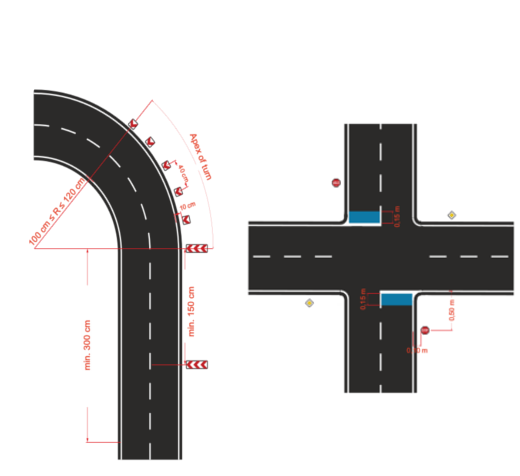
\includegraphics[width=150mm,scale=1]{./Bilder/Intersections.png}
	\caption{Left: Markings for sharp turns at Carolo-Cup.
Right: Intersections with stop lines at Carolo-Cup}
\end{figure}


%
\section*{2.2. Sobel Operator}\label{sec:Sobel Operator}
\addcontentsline{toc}{section}{2.2. Sobel Operator}
%
\begin{itemize}
 \item pers�nliche Treffen sollten gut vorbereitet werden (z.B. Fragenkatalog)
 \item Ergebnisse des Treffens und Anmerkungen des Betreuers festhalten (Notizen)
\end{itemize}

%
\section*{2.3. Edge Detection}\label{sec:Edge Detection}
\addcontentsline{toc}{section}{2.3. Edge Detection}
%
Edge detectors are essential parts of most of computer vision systems. Edge detectors decrease dramatically the 
amount of data to be processed and extract the useful part of images. They work by detecting discontinuities in 
brightness. In this project, the edge detector was used, the lanes to detect and prevent unnecessary information 
from images.

%
\section*{2.4. Hough-Transformation}\label{sec:Hough - Transformation}
\addcontentsline{toc}{section}{2.4. Hough - Transformation}
%

%
\subsection*{2.4.1. Standart Hough - Transformation}\label{sec:Standart Hough - Transformation}
\addcontentsline{toc}{subsection}{2.4.1. Standart Hough - Transformation}
%


%
\subsection*{2.4.2. Probabilistic Hough - Transformation}\label{sec:Probabilistic Hough - Transformation}
\addcontentsline{toc}{subsection}{2.4.2. Probabilistic Hough - Transformation}
%


\begin{itemize}
 \item dient zur L�sung der Problemstellung
 \item kreativste und anstrengendste Phase der Arbeit
 \item Verwendung professioneller Hilfsmittel (Programme wie Matlab oder Mathematica etc.)
 \item Treffen wenn Bedarf besteht, keine Regelm��igkeit mehr
\end{itemize}


%
\section*{2.5. Curve Fitting or Spline-Interpolation}\label{sec:Curve Fitting or Spline-Interpolation}
\addcontentsline{toc}{section}{2.5. Curve Fitting or Spline-Interpolation}
%
\begin{itemize}
 \item dient der Reorganisation der Arbeit
 \item s�mtliche Ergebnisse werden festgehalten
 \item Strukturierung und Gliederung der Ergebnisse, so dass die n�chste Phase (Schreiben) gut durchgef�hrt werden kann
 \item wenige, l�ngere Treffen zur Ergebnisbesprechung mit dem Betreuer
\end{itemize}


%
\subsection*{Ergebnissicherung}\label{sec:Ergebnissicherung}
\addcontentsline{toc}{subsection}{Ergebnissicherung}
%
\begin{itemize}
 \item alles zusammentragen was erreicht wurde $\rightarrow$ guter �berblick notwendig (S.O.)
 \item auch Programmcode ist ein Ergebnis $\rightarrow$ verst�ndlich kommentieren (Englisch)
 \item auf  Wiederverwendbarkeit von Grafiken achten (Linienst�rke, Farbe, Beschriftung, \ldots)
 \item nur noch kleine �nderungen durchf�hren (z.B. Parametereinstellungen)
\end{itemize}
\emph{Ergebnisse sollten f�r sich sprechen und f�r jeden verst�ndlich sein (ohne Erkl�rung)}


%
\section*{4. Phase: Dokumentation und Pr�sentation}\label{sec:Dokumentation}
\addcontentsline{toc}{section}{4. Phase: Dokumentation und Pr�sentation}
%
\begin{itemize}
 \item Verfassen der Arbeit und erstellen der Pr�sentation
 \item letzte Verfeinerungen an den Ergebnissen (falls notwendig)
 \item schwierigste Phase der Arbeit
 \item regelm��ige Treffen zur Korrektur des Textes / der Pr�sentation
\end{itemize}

\newpage
%
\subsection*{Wissenschaftliches Schreiben}\label{sec:Wissenschaftliches Schreiben}
\addcontentsline{toc}{subsection}{Wissenschaftliches Schreiben}
%
\begin{itemize}
 \item nicht am Layout der Arbeit aufhalten $\rightarrow$ Vorlage verwenden
 \item sehr aufwendiger Prozess von Schreiben - Verbessern - neu Schreiben - \ldots
 \item Aufwand darf nicht untersch�tzt werden (Richtwert: 1-2 Seiten / Tag)
 \item einfach erst einmal aufschreiben -  korrigiert wird dann sp�ter
 \item Struktur einer wissenschaftlichen Arbeit ist vorgegeben
 \begin{itemize}
    \item \textbf{Titelseite} mit Art der Arbeit, Titel, Namen des Autors sowie Abgabedatum.
    \item \textbf{Aufgabenstellung} wird vom Betreuer der Arbeit zur Verf�gung
      gestellt.
    \item \textbf{Erkl�rung} zur Selbst�ndigkeit. Der Text ist vorgegeben und wird bei Verwendung der Vorlage automatisch erzeugt.
    \item \textbf{Kurzfassung} der Arbeit.
      Der Umfang soll so bemessen sein, dass die englische Version
      (\textbf{Abstract}) auf die gleiche Seite passt.
    \item \textbf{Inhaltsverzeichnis} wird in \LaTeX{} durch \verb|\tableofcontents| automatisch
      erzeugt.
    \item \textbf{Symbole und Abk�rzungen}. Dieses Verzeichnis erstellt man am Besten von Hand. Die Einteilung in lateinische und griechische Symbole und Formelzeichen kann nach Bedarf ge�ndert werden (zum Beispiel nach Kapiteln oder Konzepten) oder ganz weggelassen werden
    \item \textbf{Hauptteil der Arbeit}, in einzelne Kapitel und Abschnitte unterteilen.
    \item \textbf{Anhang}. Hier k�nnen Abschnitte stehen, die beim Lesen der Arbeit
      st�ren w�rden, \zB\ Programmcode, technische Daten oder lange mathematische
      Beweise.
    \item \textbf{Literaturverzeichnis} wird entweder von Hand erstellt oder automatisch generiert (in \LaTeX{} \zB mit.
      \textsc{Bib}\TeX )
    \item \label{itm:Ordner} \textbf{Zus�tzliches Material} wie \zB\ der
      vollst�ndige Programmcode eines Software-Projekts geh�rt nicht in die Arbeit,
      sondern kann in einem separaten Ordner abgelegt werden.
 \end{itemize}
\end{itemize}
$P_\text{r�gnanz}\; O_\text{rdnung}\; E_\text{infachheit}\; M_\text{otivation}$ (einfache, kurze, strukturierte und anregende S�tze)


%
\subsection*{Verteidigung und Pr�sentation}\label{sec:Verteidigung}
\addcontentsline{toc}{subsection}{Verteidigung und Pr�sentation}
%
\begin{itemize}
 \item Inhalt der Arbeit auf ca. 10 wesentliche Punkte reduzieren
 \item je Punkt eine Folie maximal zwei
 \item je Folie 1-2 min Gespr�chszeit
 \item Struktur der Pr�sentation:
 \begin{itemize}
   \item Motivation / Einleitung (Aufgabenstellung)
   \item Grundlagen
   \item L�sungsweg
   \item Ergebnisse
   \item Zusammenfassung (und Ausblick)
 \end{itemize}
 \item komplexe Sachverhalte durch Abbildungen verdeutlichen
 \item nur Stichpunkte schreiben, keine ganzen S�tze
 \item klare, einfach nachvollziehbare Notation (z.B. bei Variablen) verwenden
 \item mehrmaliges �ben des Vortrags (z.B. vor dem Spiegel, vor der Familie, \ldots)
\end{itemize}
\emph{nichts weglassen was auf einer Folie steht, gerne zus�tzliche Dinge erw�hnen}



%
\section*{Organisatorisches}\label{sec:Organisatorisches}
\addcontentsline{toc}{section}{Organisatorisches}
%
\begin{itemize}
 \item Bewertung
 \begin{itemize}
   \item Arbeitsstil: 40\% - Selbst�ndigkeit, Verst�ndnis, Kreativit�t, Flei�, Zusammenarbeit mit Betreuer, Systematik
   \item Ergebnisse: 20\% - Qualit�t, Nutzbarkeit, Innovations-, Erf�llungsgrad
   \item Ausarbeitung: 30\% - Aufbau, �u�ere Form, Sprache, Grundlagen, Vollst�ndigkeit
   \item Vortrag: 10\% - Inhalt, Stil, Folien, Vorf�hrung, Diskussion
 \end{itemize}
 \item jeder Studierende sollte an mindestens einem Regelungstechnischen Seminar teilnehmen
 \item Abgabetermin ist ein fixer Termin $\rightarrow$ Pr�fungsleistung (Durchfallen m�glich)
 \item jeder Studierende erh�lt auf Wunsch einen eigenen Account f�r unsere Rechner (Passwort legt Admin fest)
 \item zur Erstellung der Ausarbeitung und der Pr�sentation wird die Verwendung des Textsatzprogramms LaTeX empfohlen, das Template f�r die Ausarbeitung erhaltet Ihr vom Betreuer
\end{itemize}


%
\section*{Allgemeines zu Hilfsmitteln bei der Erstellung und Bearbeitung}\label{sec:Allgemeines}
\addcontentsline{toc}{section}{Allgemeines zu Hilfsmitteln bei der Erstellung und Bearbeitung}
%
\begin{itemize}
 \item es gibt viele B�cher die bei der Erstellung von wissenschaftlichen Arbeiten helfen
 \item viele verwendete Programme bieten ausf�hrliche Hilfen an (z.B. Matlab, Mathematica)
 \item bei Problemen immer zuerst in der Hilfe schauen, dann "googlen", dann Betreuer fragen
\end{itemize}


%
\subsection*{Empfohlene Programme}\label{sec:Empfohlene Programme}
\addcontentsline{toc}{subsection}{Empfohlene Programme}
%
\begin{itemize}
 \item Literaturdatenbank $\rightarrow$ JabRef (http://jabref.sourceforge.net/)
 \item Ausarbeitung und Pr�sentation $\rightarrow$ \LaTeX / PowerPoint
 \item Simulation und Regelungstechnik $\rightarrow$ Matlab/Simulink
 \item symbolische und numerische Berechnungen $\rightarrow$ Mathematica
 \item Plots $\rightarrow$ \texttt{pgfplots}
 \item Blockschaltbilder $\rightarrow$ \texttt{TikZ}
\end{itemize}

%
\chapter{Related Works}\label{cha:Related Works}

In the automotive industry, one area of particular research interest is autonomous driving, and within this area, lane detection an important component being actively researched. As can be attested by the various projects carried out and scientific papers written on the subject, many different methods can be used in lane detection, each with its own advantages and disadvantages. In terms of disadvantages, some are only able to detect straight lines, for example, while others are not robust in rainy weather or in different light conditions. Some papers also compare the results of different lane detection projects. One of them is from Ammu M Kumar and Philomina Simon from India, which compares some lane detection projects conducted between 2003 and 2014.\cite{Review_of_Lane_Detection}
 
According to the literature, one of the methods used most often for lane detection is the 'Hough Transformation'. But there are also some other methods like 'Haar like features', 'Random sample consensus (RANSAC)' or 'Artificial Neural Network(ANN)'. In this chapter, some different methods will be described in order to provide an overview of the methods used in lane detection.

One important algorithm for lane detection was developed by Mohamed Aly, and was also used by Nicolas Acero Sepulveda, who did his bachelor's thesis in the area of lane detection at the Technical University of Darmstadt in 2016.\cite{Bachelorthesis_Nicolas} In the beginning of this method, with the aid of Inverse Perspective Mapping(IPM) algorithm, the view is changed from the camera view to the top view. By doing so, the perspective effect is avoided. For the top view frame, the Gaussian and threshold filters are used to filter noise. This method is not very different from Method 2 used in this master's thesis. However, in Aly's algorithm the Random sample consensus (RANSAC) algorithm was used for lane detection, while in this master's thesis, the Probabilist Hough Transformation was used.

In another method\cite{An_Efficient_Lane_Detection} for lane detection, the 'Haar like features' algorithm was used to obtain potential lane points. According to authors, the processing time of this method is approximately 0.12 ms and the detection rate is 90.16\%. It is one of the fastest algorithms for lane detection. In this method, because of the perspective effect, the lanes appear diagonal, so a diagonal directional filter called the 'steerable filter' is used, and then the 'Haar like features' algorithm is applied. After this process, the maximum responses are obtained, which are the left and right lanes.

An another robust method\cite{A_Fast_and_Robust_Approach}, which was developed at the Technical University of Braunschweig, was tested successfully in a competition for autonomous automobiles in 2007 called the 'DARPA Urban Challenge'. The 'DARPA Urban Challenge' is different than Carolo-Cup, because the Carolo-Cup is for a 1:10 concept of an automated vehicle, but the DARPA Urban Challenge is for real vehicles. In this project, the IPM technique was used and instead of the RGB color space, the HSV color space was used, because this format is much more robust under different light conditions. In this project, like in Aly's project, the RANSAC algorithm was used. According the paper written for this project, just ten frames per second can be processed and this project needs to have a modern graphics card.


%
\chapter{Implementation}\label{cha:Implementation}
%
\section*{3.1.Test Track}\label{sec:Test Track}
\addcontentsline{toc}{section}{3.1.Test Track}

As before mentioned, medium-term goal of this master thesis is attending to the Carola-Cup at Braunschweig University 
so the test truck was prepaid in the Carola-Cup properties by Nicolas Acero Sepulveda, who did his bachelor thesis also
with this model auto. For this test truck, two black PVC floor carpets were used and on these floor carpets, the lanes 
of the truck were made by using white electrical tape. The straight part of the truck was made on one of these PVC 
floor carpet and the curved part of truck was made on second PVC floor carpet. The straigt part of the truck is 
approximately 2 meters long and the curve radius of the curved part of test truck is approximately 1 meter. This curve 
is the tightest curve at Carola-Cup so with this test truck can be tested the worst case situation. In the Carola-Cup 
competition, the truck is much more bigger but for testing this master thesis, we don't need to build bigger test truck.


%
\section*{3.2.Hardware}\label{sec:Hardware}
\addcontentsline{toc}{section}{3.2.Hardware}

%
\subsection*{3.2.1. Model Auto}\label{sec:Model Auto}
\addcontentsline{toc}{subsection}{3.2.1. Model Auto}

During the course of this master thesis, a model automobile was being used which was prepared for the Projectseminar 
Echtzeitsysteme at Technical University of Darmstadt. The chassis, steering mechanism, power train, and engine control 
were derived from the model-building of a Japanese company, Tamiya. The maximum velocity of the model automobile is 
approximately 1 m/s and the minimum steering radius is around 90 cm. 

%

\subsection*{3.2.2. Microcontroller and Main Board}\label{sec:Microcontroller and Main Board}
\addcontentsline{toc}{subsection}{3.2.2. Microcontroller and Main Board}

In this model auto, there is a microcontroller and a main board. The microcontroller is used for controlling steering 
and receiving the measurements from ultrasonic sensors and hall effect sensors. The 16-bit microcontroller is from 
MB96300 series from Fujitsu company.

The main board on the model car is from PD10BI-MT ThinMini-ITX series from MiTAC company. This main board communicate 
with the microcontroller over via UART interface through USB connection. On this main board, there is an Intel 
Quadcore-Processor and an Intel HD Graphics card. Furthermore, there is a 8 GB DDR3-1600 RAM and 1Gbit/s Ethernet, VGA 
and HDMI connections.
%

\subsection*{3.2.3. Camera}\label{sec:Camera}
\addcontentsline{toc}{subsection}{3.2.3. Camera}

The camera is one of the main components of lane detection and accordingly, autonomous driving. For this thesis, I had 
to research the most suitable camera because all cameras have different properties.

At the beginning of the Projectseminar Echtzeitsysteme, the Logitech C270 HD Webcam was being used. The resolution of 
the camera is 1280x960 pixels and the Frame per Second (FPS) value is 30 Hertz (Hz) at a 640x480 pixel resolution. 
The field of View (FOV) is just 60 degrees. The problem with this camera is that if there is a curve, the camera 
cannot see all of the lanes, and thus is not very suitable for lane detection. When I started my master thesis, there 
was a Kinect v2 camera on the model car.  The Kinect v2 camera was developed by Microsoft and released in 2013. This 
camera has a depth sensor with a resolution of 512x424 pixels and its FOV is 70x60 degrees. The FPS value is 30 Hz at 
a 512x424 pixel resolution. This camera also has a color camera with resolution of 1920x1080 pixels and a FOV of 
84.1x53.8 degrees. The FPS value is 30 Hz at a 1920x1080 pixel resolution. This camera had two main disadvantages for 
this master thesis. The first disadvantage is the FOV value of camera. This value is better than the value of Logitech 
C270 camera but it is still not enough for curve lane detection. The second main disadvantage is the location of the 
color camera. The color camera of this camera is not in the middle of camera, but rather, on the right. This is a 
disadvantage for us because when there are curves going left as opposed to right, the camera is unable to see the 
left and even perhaps the middle lane of the truck. Thus, this is problematic for lane detection.

Due to these reasons, I had to choose a camera which has a sufficiently high FOV value. After doing research, I decided 
that the Genius Widecam F100 camera is the best choice for this master thesis because this camera has a FOV value of 
120 degrees and it can also be used with the Linux Operating System. The resolution of this camera is 1920x1080 pixels 
and the FOV value is 120 degrees. The FPS is 30 Hz at a 1920x1080 pixel resolution. With this camera, it is possible 
to detect most if not all lanes, including when there are curves. 

\begin{figure}
	\centering
	\hspace*{0cm}   
	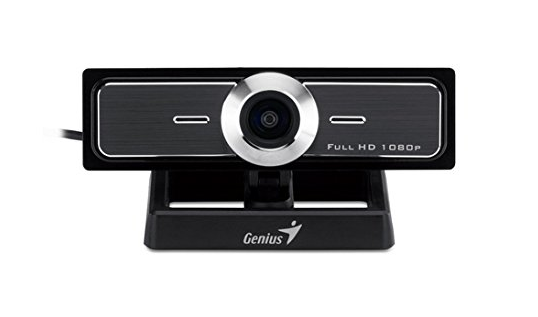
\includegraphics[width=150mm,scale=1]{./Bilder/Genius_F100_camera.png}
	\caption{Genius 120-degree Ultra Wide Angle Full HD Conference Webcam(WideCam F100) }
\end{figure}


%
\section*{3.3.Software}\label{sec:Software}
\addcontentsline{toc}{section}{3.3.Software}
%



%
\chapter{Evaulation and Discussion}
\label{cha:Evaulation and Discussion}

%Dieses Kapitel gibt allgemeine Hinweise zur Erstellung einer wissenschaftlichen Arbeit mit dem Textsatzprogramm \LaTeX. Es ist inhaltlich identisch mit dem vorherigen Kapitel und enth�lt zus�tzlich die \LaTeX-spezifischen Befehle, die bei der Umsetzung der Hinweise hilfreich sein k�nnten.

%Wird die Arbeit \emph{nicht} mit \LaTeX\ erstellt, sollte das vorherige Kapitel gelesen werden.

%Besonderes Augenmerk sollte auf Abschnitt~\ref{sec:Latex-Zitieren}, \textbf{Zitate und korrekte Zitierweisen} gelegt werden.

Dieses Kapitel gibt allgemeine Hinweise zur Erstellung einer wissenschaftlichen Arbeit mit dem Textsatzprogramm \LaTeX. Das Kapitel sollte auch von Studierenden gelesen werden, die sich gegen eine Erstellung der Arbeit mit \LaTeX\ entschieden haben. Da das Layout der Arbeit in diesem Fall gem�� den TUD Designvorgaben zus�tzlich selbst erstellt werden muss, dient die vorliegende Anleitung auch als Vorlage.

%Wird die Arbeit \emph{nicht} mit \LaTeX\ erstellt, sollte das vorherige Kapitel gelesen werden.

%Besonderes Augenmerk sollte auf Abschnitt~\ref{sec:Latex-Zitieren}, \textbf{Zitate und korrekte Zitierweisen} gelegt werden.

\section{Editor}
F�r LATEX gibt es eine Vielzahl von freien und kommerziellen Texteditoren. Das \textsc{TeXnicCenter} ist ein freier open-source Editor, der sich bei uns am Institut bew�hrt hat. Eine Anleitung zur Einrichtung des \textsc{TeXnicCenter} befindet sich in dieser zip-Datei.

\section{Rechtschreibung}

Studentische Abschlussarbeiten am IAT sind nach \emph{neuer} deutscher
Rechtschreibung zu verfassen. Die wesentlichen �nderungen betreffen die Gro�-
und Kleinschreibung sowie die Getrennt- und Zusammenschreibung,
siehe~\cite{Duden}. Das offensichtlichste Merkmal ist die neue
\glqq �\grqq-Regel: Nach kurzem Vokal steht jetzt \emph{immer} \glqq ss\grqq\ (wie in Abschluss),
nach langem Vokal \glqq �\grqq\ (wie in Fu�). Die neue deutsche Rechtschreibung wird in
\LaTeX\ mit dem Paket \verb|babel| �ber die Option \verb|ngerman| aktiviert.

Im Internet findet man unter \verb|http://www.duden.de/| einen Crashkurs zur
neuen deutschen Rechtschreibung.


\section{Zitate und korrekte Zitierweise}
\label{sec:Latex-Zitieren}

Zitate sind w�rtliche oder sinngem��e Wiedergaben von Gedanken, Ideen oder Meinungen anderer Autoren. Werden Ideen oder Inhalte aus Quellen w�rtlich oder sinngem�� in die eigene Arbeit �bernommen, besteht die \textbf{Pflicht}, diese zu kennzeichnen. Wird dies unterlassen, liegt ein \textbf{T�uschungsversuch} (Plagiat) vor und die Arbeit kann als \textbf{nicht bestanden} bewertet werden.

Laut � 38 Abs. 2 der \emph{Allgemeinen Pr�fungsbestimmungen} liegt \glqq\ [...] ein T�uschungsversuch [...] vor, wenn eine falsche Erkl�rung nach �� 22 Abs. 7, 23 Abs. 7 abgegeben worden ist oder ein anderes Werk, eine Bearbeitung eines anderen Werkes, eine Umgestaltung eines anderen Werkes ganz oder teilweise in der Pr�fungsarbeit wiedergeben werden, ohne dieses zu zitieren (Plagiat).\grqq~\cite{APB}

\subsection*{Zitierf�higkeit}
Zitierf�hig sind nur ver�ffentlichte Werke aus allgemein zug�nglichen Quellen (B�cher, Artikel, \etc). Quellen, bei denen die Verf�gbarkeit nicht garantiert werden kann (Internetquellen) oder der Urheber nicht klar nachvollziehbar ist (Wikipedia, o.\,�\,.), sind problematisch und sollten m�glichst vermieden werden. Wird doch solch eine Quelle zitiert, ist die aktuelle Version zum Zeitpunkt des Zitates beizulegen.

\subsection*{W�rtliche Zitate}
W�rtliche Zitate in ingenieurwissenschaftlichen Arbeiten sind un�blich. Sollte doch ein w�rtliches Zitat in die Arbeit �bernommen werden, muss dieses buchstaben- und zeichengetreu, inklusive eventueller Rechtschreibfehler �bernommen werden. Das w�rtliche Zitat wird in Anf�hrungszeichen eingefasst.

\subsection*{Sinngem��e Zitate}
Weit h�ufiger werden in wissenschaftlichen Arbeiten Ideen oder Meinungen anderer Autoren sinngem�� �bernommen. Diese m�ssen durch einen Verweis auf die Quelle gekennzeichnet werden. Durch die Position des Verweises muss der Umfang der sinngem��en �bernahme klar hervorgehen.

\subsection*{Quellenangaben im Literaturverzeichnis}
F�r die Darstellung der Verweise, als auch f�r die Darstellung der Quellen im Literaturverzeichnis gibt es verschiedene Zitierweisen. �blich sind die Harvard-Variante mit Autor und Ver�ffentlichungsjahr in runden Klammern, wie zum Beispiel (Isermann, 2001) oder eine fortlaufende Nummerierung in eckigen Klammern, wie in dieser Vorlage. Die Sortierung des Literaturverzeichnisses kann alphabetisch oder nach dem Erscheinen der Verweise erfolgen. Das \texttt{bibgerm} Paket erm�glicht verschiedene (im Deutschen �bliche) Zitierweisen.

Ein Verweis wird mit \verb|\cite{...}| eingef�gt und mit einem festen Leerzeichen \verb|~| mit dem vorherigen Wort getrennt. Schlie�t der Verweis einen Satz ab, folgt der Punkt \emph{hinter} dem Verweis.

F�r die Erstellung des Literaturverzeichnisses bietet sich die Erweiterung \textsc{Bib}\TeX\ an. Das Literaturverzeichnis kann per Hand oder automatisch erstellt werden. Viele Literaturverwaltungsprogramme, wie zum Beispiel \textsc{JabRef} erm�glichen den direkten Export der Datenbank nach \textsc{Bib}\TeX.


\section{Gliederung des Dokuments}
\label{sec:Latex-Gliederung}


Im Inhaltsverzeichnis wird die Gliederung der Arbeit dargestellt. Die �berschriften und Seitenangaben der Kapitel, Unterkapitel und Abschnitte m�ssen mit den Elementen im Inhaltsverzeichnis �bereinstimmen. �berschriften sind kurz und pr�gnant zu formulieren und d�rfen keine vollst�ndigen S�tze sein. Gibt es Unterpunkte in der Gliederung, so m�ssen immer mindestens zwei davon existieren und inhaltlich auf der gleichen Ebene sein. Die einzelnen Punkte des Inhaltsverzeichnis m�ssen nummeriert werden. Die �bersichtlichkeit des Inhaltsverzeichnisses kann durch Einr�cken der Unterpunkte erh�ht werden.

Das Inhaltsverzeichnis wird in \LaTeX\ automatisch erstellt.
Innerhalb der einzelnen Kapitel \verb|\chapter{...}| werden weitere
Unterteilungen mit den Befehlen \verb|\section{...}|, \verb|\subsection{...}|
usw.\ vorgenommen. Werden diese mit einem \verb|*| versehen, dann erh�lt der
jeweilige Abschnitt keine Nummer und erscheint nicht im Inhaltsverzeichnis. Dies
kann in manchen F�llen n�tzlich sein.

Um eine korrekte Darstellung des Inhaltsverzeichnisses
zu erhalten, muss ggf. mehrmals hintereinander kompiliert werden, da sich aufgrund von
Gleitobjekten Seitenzahlen �ndern k�nnen. Dreimaliges Kompilieren reicht in der Regel.

Bei Bildern und Tabellen, die in eine \verb|figure|- bzw.\ \verb|table|-Umgebung
eingeschlossen sind, handelt es sich um sog.\ \emph{Gleitobjekte}, d.\,h.\ sie
erscheinen nicht an der Stelle, an der sie eingebunden werden, sondern oben oder
unten auf einer Seite, siehe \zB\ Tabelle~\ref{tab:Sonderzeichen} auf
Seite~\pageref{tab:Sonderzeichen}. Optional k�nnen in \verb|[]| noch
Positionierungsw�nsche angegeben werden. Mit dem Befehl \verb|\caption{...}|
erhalten Bilder eine \emph{Unterschrift} und Tabellen eine \emph{�berschrift}.

Kapitel, Abschnitte, Bilder, Tabellen und Gleichungen k�nnen mittels
\verb|\label{...}| benannt werden. Dadurch ist es m�glich, sie sp�ter mit
\verb|\ref{...}| oder \verb|\pageref{...}| zu referenzieren. Es empfiehlt sich,
den Namen (Labels) eine Markierung voranzustellen, aus der hervorgeht, um
welches Objekt es sich handelt. �blich sind \verb|cha:| f�r \glqq Chapter\grqq,
\verb|sec:| f�r \glqq Section\grqq, \verb|fig:| f�r \glqq Figure\grqq,
\verb|tab:| f�r \glqq Table\grqq\ und \verb|eq:| f�r \glqq Equation\grqq. Ein
Bild benennt man also \zB\ mit \verb|\label{fig:Ausgangssignal}|.

\section{Bilder}\label
{sec:Latex-Bilder}

Wenn m�glich, sollten Bilder als Vektorgrafik eingebunden werden, damit sichergestellt werden, dass alle Details beim Ausdrucken erhalten bleiben. Es ist dabei auf eine ausreichende Strichst�rke zu achten. Ebenfalls sollten die im Bild verwendete Schrift die gleiche sein, wie im �brigen Dokument.

Werden doch Pixelgrafiken verwendet, so ist die richtige Wahl der Aufl�sung von besonderer Bedeutung. Einerseits sollten die Bilder auf dem ausgedrucken Dokument gut aussehen, andererseits aber auch eine z�gige Bildschirmdarstellung und kleine Dateigr��e erm�glichen.


F�r die Erstellung von Plots eignet sich das \LaTeX-Paket \texttt{PGFPLOTS} sehr gut. Eine Anleitung zu diesem Paket befindet sich in dieser zip-Datei. In Anhang~\ref{cha:Anhang-Grafiken} sind weitere geeignete Programme zur Erstellung von Bildern und Plots mit ihren Eigenschaften aufgelistet.

Eine Grafik l�sst sich am einfachsten mit dem Befehl \verb|\includegraphics{}|
aus dem \verb|graphicx|-Paket einbinden. Eine vollst�ndige Beschreibung des
Befehls und weiterer n�tzlicher Grafikbefehle findet man in der Dokumentation
des \verb|graphicx|-Pakets. Diese liegt -- wie die Beschreibung aller anderen
\LaTeX-Pakete -- im \verb|doc|-Verzeichnis des \TeX-Systems. In welchem Format
\verb|graphicx| die Grafiken ben�tigt, h�ngt davon ab, ob man \TeX\ in
Verbindung mit Dvips verwendet oder stattdessen pdf\TeX, siehe
Anhang~\ref{cha:TexSystem}.

F�r \textbf{\TeX/Dvips} (empfohlen) m�ssen alle Grafiken im
\emph{Encapsulated-PostScript}-Format (\verb|*.eps|) vorliegen. EPS-Dateien
lassen sich aus praktisch jeder Software erzeugen und k�nnen sowohl Vektor- als
auch Pixelgrafiken enthalten -- zus�tzlich sind auch Preview-Grafiken m�glich,
was aber in der \TeX-Welt im Allgemeinen nicht erforderlich ist.

\textbf{pdf\TeX} verarbeitet dagegen Grafiken im \emph{Portable-Document-Format}
(\verb|*.pdf|) sowie die Pixelformate JPEG und PNG. Den direkten Export von
PDF-Grafiken bieten derzeit zwar nur wenige Programme an, sie lassen sich aber
einfach aus dem EPS-Format mit Hilfe des Acrobat Distiller oder Ghostscript
erzeugen.

Bilder m�ssen zentriert sein (\verb|\centering|) und eine Bild\emph{unterschrift} (\verb|\caption{...}|) besitzen. Um auf eine Abbildung zu referenzieren, kann auch sie mit einem \verb|\label{fig:...}| versehen werden. Nur in besonderen Ausnahmef�llen sollten Bilder mit Text umflossen werden. Wurden Abbildungen einer Quelle entnommen, muss dies entsprechend mit einem Verweis auf die Quelle im Literaturverzeichnis gekennzeichnet werden. Werden Abbildungen eine Quelle nachempfunden, angepasst oder abge�ndert, ist dies mit dem Zusatz \glqq in Anlehnung an...\grqq\ oder �hnlich anzugeben.

\begin{figure}[htp]
	\centering
	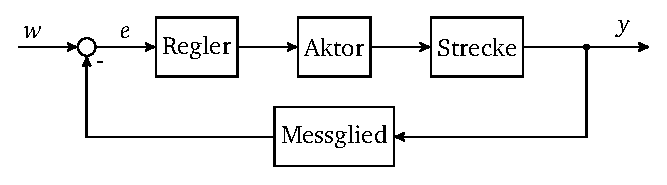
\includegraphics{./Bilder/BSB_Beispiel-ext}
	\caption{Standard-Regelkreis; Bild erstellt mit \texttt{TikZ}}
\end{figure}

Generell ist die Arbeit (und insbesondere die Grafiken) so zu gestalten, dass
sie auch schwarzwei� gedruckt werden kann. Farbige Fotos und Screenshots
verursachen dabei i.\,Allg.\ keine zus�tzlichen Probleme. Werden jedoch \zB\
farbige Kurven in einem Diagramm dargestellt, hat dies folgende Konsequenzen:
\begin{itemize}
\item Keine zu hellen Farben f�r die Linien verwenden, da diese sonst beim
  Drucken nicht zu erkennen sind. RGB-Gr�n $(0,1,0)$ ist tabu!
\item Bei mehreren Kurvenverl�ufen darf deren Farbe nicht das einzige
  Unterscheidungsmerkmal sein: Entweder sind unterschiedliche Linienformen zu
  verwenden oder die Kurven im Diagramm beschriften.
\end{itemize}

Bei der Erstellung von Plots ist unbedingt die \href{http://de.wikipedia.org/wiki/DIN_461}{\texttt{DIN 461 Grafische Darstellung in Koordi}}\texttt{-} \href{http://de.wikipedia.org/wiki/DIN_461}{\texttt{natensystemen}} zu beachten. Hilfreich in diesem Zusammenhang und �berhaupt f�r die korrekte Schreibweise von Zahlen und Einheiten im Flie�text und in Formeln sind die Hinweise der TU-Chemnitz: \verb+www.tu-chemnitz.de/physik/FPRAK/Grundsatz/Literatur/si_v1.pdf+.

\section{Tabellen}

Tabellen m�ssen ebenfalls zentriert sein und besitzen eine zentrierte Tabellen\emph{�berschrift} (\verb|\caption{...}|). Hier gelten die gleichen Regeln zur Quellenangabe wie bei den Bildern. Ein Referenzieren wird auch hier mit \verb|\label{tab:...}| erm�glicht.

Damit Tabellen \glqq sch�n\grqq\ aussehen, empfiehlt es sich, einige Grundregeln zu beachten. Es gilt das Prinzip: \emph{weniger ist mehr.} So sollte auf die Verwendung von senkrechten Linien verzichtet werden und nur wichtige Zeilen, wie zum Beispiel �berschriften, Sinnabschnitte, Unterpunkte, \etc mit horizontalen Linien getrennt werden. Das Paket \verb|booktabs| stellt Linientypen f�r den Kopf und Fu� einer Tabelle zur Verf�gung.


\begin{table}[htb]
\begin{center}
\caption{Parameter\footnotemark}
\label{tab:Systemparameter}
\begin{tabular}{ccccp{3mm}cccc}
	\toprule
	& Ref. & Mod. & Einheit & & & Ref. & Mod. & Einheit\\
	\cmidrule(r){1-4}									\cmidrule(l){6-9}
	$m_1$ & 4{,}0 & 4{,}63 & \unit{kg} &	
		&$d_1$ & 0 & 0 & \unit{\frac{N\,m\,s}{rad}}\\[1mm]
	$m_2$ & 10{,}1 & 11{,}15 & \unit{kg} &	
		&$d_2$ & 0 & 0 & \unit{\frac{N\,m\,s}{rad}}\\[1mm]
	$m_3$ & 45{,}7 & 42{,}5 & \unit{kg} &	
		&$l_1$ & 0{,}5 & 0{,}45 & \unit{m}\\[1mm]
	$J_1$ & 0{,}967 & 0{,}993 & \unit{kg\,m^2} &	
		&$l_2$ & 1{,}5 & 1{,}59 & \unit{m}\\[1mm]
	$J_2$ & 0{,}571 & 0{,}599 & \unit{kg\,m^2} &
		&$\varphi_{1,0}$ & 100 & 98{,}5 & \unit{\degree}\\[1mm]
$g$ & 9{,}81 & 9{,}81 & \unit{\frac{m}{s^2}} &
		&$\varphi_{2,0}$ & {5} & {4.66} & \unit{\degree} \\
	\bottomrule
\end{tabular}
\end{center}
\end{table}
\footnotetext{Eine sch�nere Formatierung der Tabelle (Ausrichtung am Trennzeichen, etc.) erlaubt das \texttt{siunitx}-Paket, welches sich aber mit irgendwas in der Vorlage bei�t (nur Warnmeldungen, aber trotzdem...) }

\section{Mathematische Formeln}

Mathematische Formeln, wie 
\begin{equation}
  \label{eq:Allgemein-Approx}
  \int_0^\infty g(x)\,\mathrm{d}x\approx\sum_{i=1}^n w_i\mathrm{e}^{x_i} g(x_i)
\end{equation}
werden einger�ckt linksb�ndig dargestellt und nur dann nummeriert, wenn auf sie im Text verwiesen wird. F�r eine bessere Lesbarkeit ist es sinnvoll Gleichungen als Bestandteil des Satzes zu verwenden, so wie mit Gleichung~\eqref{eq:Allgemein-Approx}. Die Referenzierung einer erst sp�ter aufgef�hrten Gleichung sollte vermieden werden.

\emph{Alle} mathematischen Ausdr�cke (auch wenn es nur einzelne Zeichen sind)
werden im mathematischen Modus \verb|$...$| geschrieben, damit sie in der
richtigen Schrift erscheinen. Hier gilt die Faustregel, dass gew�hnliche
mathematische Gr��en \emph{kursiv} geschrieben werden, Ausdr�cke mit
konventioneller (feststehender) Bedeutung dagegen in normaler (steiler,
aufrechter) Schrift, siehe~\cite{DIN1338}. Es sind insbesondere Einheiten,
Standardfunktionen und -operatoren sowie mathematische Konstanten steil zu
schreiben,
\begin{displaymath}
  \mathrm{e}^{ax}\;,\qquad a+\mathrm{j}b\;,\qquad
  \int_{t=0}^{t=1\,\mathrm{s}} f(t)\cdot\sin(\omega t)\,\mathrm{d}t\;.
\end{displaymath}
Da der mathematische Modus zun�chst alle Gr��en \emph{kursiv} setzt, m�ssen
Ausdr�cke, die in aufrechter Schrift erscheinen sollen, mit dem Befehl
\verb|\mathrm{...}| gekennzeichnet werden; bei Textteilen innerhalb einer Formel
verwendet man besser \verb|\mbox{...}| oder \verb|\text{...}| (aus dem
\verb|amsmath|-Paket). F�r Standardfunktionen werden von \LaTeX\ die
entsprechenden Befehle \verb|\sin|, \verb|\log|, \verb|\max| usw.\ zur Verf�gung
gestellt. Konsequenter Weise muss dieses Prinzip auch auf Indizes angewendet
werden, also \zB
\begin{displaymath}
  \sum_{i,\,j}a_{ij}\,\sin(ijx)\;,\qquad\mbox{aber:}\qquad
  K_\mathrm{Regler} = 0{,}5\;.
\end{displaymath}
Als Ausnahme von der o.\,g.\ Faustregel werden gro�e griechische Buchstaben
meist \emph{nicht} kursiv geschrieben, so auch im mathematischen Modus von
\LaTeX. Matrizen und Vektoren werden in \textbf{fetten} Buchstaben gesetzt.
Damit sie sich besser von den �brigen Symbolen abheben, werden auch sie nicht
\textbf{\emph{fett-kursiv}} sondern \textbf{fett-steil} geschrieben. Dazu
definiert man zweckm��igerweise im Vorspann des Dokuments den Befehl
\begin{center}
\verb|\newcommand{\mat}[1]{{\ensuremath{\boldsymbol{\mathrm{#1}}}}}|\,,
\end{center}
den man dann sowohl f�r Matrizen (Gro�buchstaben, \zB\ \verb|\mat{A}|) als
auch f�r Vektoren (Kleinbuchstaben, \zB\ \verb|\mat{x}|) verwenden kann.
\begin{displaymath}
  \mat{A}=\left(\begin{array}{ccc}
    a_{11} & \ldots & a_{1n} \\
    \vdots & \ddots & \vdots \\
    a_{n1} & \ldots & a_{nn}
  \end{array}\right)\;,\qquad
  \mat{x}=\left(\begin{array}{@{}c@{}} x_1 \\ x_2 \end{array}\right)\;,\qquad
  \mat{\beta}^\mathrm{T}=(\beta_1,\,\ldots,\,\beta_m)
\end{displaymath}

Chemische Formelzeichen schreibt man grunds�tzlich in aufrechter Schrift.
Variable Gr��en sind aber auch hier kursiv:
\begin{displaymath}
  \mathrm{H_2 O}\;,\qquad
  \mathrm{NO}_x\;,\qquad
  \mathrm{Fe_2^{2+}Cr_2^{\vphantom{2+}}O_4^{\vphantom{2+}}}
\end{displaymath}


Beim Referenzieren von Gleichungen muss diese nummeriert werden. Ist die Gleichung
\begin{equation}
  \label{eq:Approx}
  \int_0^\infty g(x)\,\mathrm{d}x\approx\sum_{i=1}^n w_i\mathrm{e}^{x_i} g(x_i)
\end{equation}
mit \verb|\label{eq:Approx}| bezeichnet, erzeugt die Referenz \verb|\eqref{eq:Approx}| den Ausdruck \glqq \eqref{eq:Approx}\grqq. Kapitel, Abschnitte, Bilder und Tabellen bekommen keine Klammern, also \zB\
\verb|Kapitel~\ref{cha:Intro}| f�r \glqq Kapitel~\ref{cha:Intro}\grqq. Es ist
darauf zu achten, ob es sich um \emph{Kapitel} oder \emph{Abschnitte} handelt.
Vor \verb|\ref{...}| steht ein \emph{festes} Leerzeichen~\verb|~|, damit dort
kein Umbruch erfolgen kann. Literaturangaben werden mit \verb|\cite{...}|
anstelle von \verb|\ref{...}| referenziert.

Werden Gleichungen oder Listen in den laufenden Text eingef�gt, darf dazwischen
kein Absatz (d.\,h.\ eine Leerzeile im Quelltext) sein. Um den Quelltext
besser zu gliedern, kann an dieser Stelle eine Zeile mit einem \verb|%|-Zeichen
eingef�gt werden. Eine Leerzeile darf nur dann im Quelltext stehen, wenn auch
wirklich ein Absatz erw�nscht ist. Der Zeilentrenner \verb|\\| erzeugt �brigens
keinen Absatz und darf im laufenden Text �berhaupt nicht vorkommen.


\section{Auszeichnungen und Hervorhebungen}

Wichtige Begriffe werden durch eine andere Schrift hervorgehoben (ausgezeichnet).
Man unterscheidet dabei integrierte und aktive Auszeichnungen.
Integrierte Auszeichnungen sollen erst beim Lesen wahrgenommen werden, sich aber
ansonsten in den Text eingliedern. Die typische Form einer integrierten
Auszeichung ist die \emph{kursive} Schrift, die mit \verb|\textit{...}| oder
\verb|\emph{...}| erzeugt wird. Aktive Auszeichnungen sollen dagegen sofort beim
Betrachten der Seite auffallen. Der wichtigste Vertreter ist hier die
\textbf{fette} Schrift, die man durch Verwendung von \verb|\textbf{...}| erh�lt.
In wissenschaftlichen Arbeiten werden vorwiegend integrierte Auszeichnungen
benutzt.

Grunds�tzlich sollte bei Auszeichnungen immer nur \emph{ein} Attribut ge�ndert
werden, also \emph{nicht} gleichzeitig \emph{\underline{\textbf{fett, kursiv und
unterstrichen}}}. Programmcode und Befehle setzt man �blicherweise mit
\verb|\texttt{...}| oder \verb+\verb|...|+ in \texttt{Schreibmaschinenschrift},
Namen gelegentlich mit \verb|\textsc{...}| in \textsc{Kapit�lchen}. F�r manche
Bezeichnungen kommt eine \textsf{\textbf{fette serifenlose}} Schrift
\verb|\textsf{\textbf{...}}| in Frage. Hier m�ssen ausnahmsweise \emph{zwei}
Attribute ge�ndert werden, da sich die \textsf{serifenlose} Schrift zu wenig vom
�brigen Text abhebt.

\glqq Anf�hrungszeichen\grqq\ (siehe Abschnitt~\ref{sec:Sonderzeichen}) sind
sparsam zu verwenden, \zB\ bei umgangssprachlichen Begriffen oder w�rtlichen
Zitaten. \underline{Unterstreichen} und \mbox{S\,p\,e\,r\,r\,e\,n} sollen
�berhaupt nicht benutzt werden. Es ist wichtig, sich zu Beginn der Arbeit
zu �berlegen, welche Begriffe in welcher Schrift
gesetzt werden, und dies konsequent einzuhalten.


\section{Einbinden von Quellcode}

Wird Quellcode (MATLAB, C, \ldots) in der Arbeit angegeben, ist grunds�tzlich
eine Monospace-Schriftart zu verwenden, da nur so die Lesbarkeit des Codes
gew�hrleistet werden kann.

Quellcode (MATLAB, C, \ldots) kann auf verschiedene Arten eingebunden werden.
Allgemein sollte mittels \verb|\linespread{1}| der urspr�ngliche
\LaTeX-Zeilenabstand benutzt werden. Manchmal kann es auch erforderlich sein,
die Schrift zu verkleinern oder notfalls sogar die Seiten im Querformat zu
beschreiben. Im laufenden Text sollten nur kleinere Code-Fragmente abgedruckt
sein, l�ngere Programme geh�ren grunds�tzlich in den Anhang oder in einen
separaten Ordner.

Die einfachste M�glichkeit zum Einbinden von Quellcode ist die \verb|verbatim|-
bzw.\ die \verb|verbatim*|-Umgebung. Der Code wird in
Schreibmaschinenschrift \emph{exakt} (inkl.\ aller Leer- und Sonderzeichen) so
wiedergegeben, wie er im \LaTeX-Quelltext steht.

Komfortablere M�glichkeiten bietet das \verb|listings|-Paket, \zB\
Syntax-Highlighting mit verschiedenen Schriften oder das Einbinden externer
Dateien. Die Umschaltung auf den einfachen Zeilenabstand muss aber von Hand
erfolgen, \zB\ mittels\\[\parskip]
\hspace*{2em}\verb|\lstset{\basicstyle=\linespread{1}\selectfont}|


\section{Abst�nde und Sonderzeichen}\label{sec:Sonderzeichen}

\LaTeX\ interpretiert ein Leerzeichen \verb*| | im Quelltext als normalen
Wortzwischenraum. Nach Befehlen wird es jedoch ignoriert, da es dort nur das
Ende des Befehls kennzeichnet. Soll \zB\ in dem Satz \glqq\TeX\ ist
toll!\grqq\ nach \glqq\TeX\grqq\ ein Leerzeichen erscheinen, dann muss im
Quelltext entweder \verb*|\TeX\ | oder \verb|\TeX{}| geschrieben werden. Im
ersten Fall wird durch \verb*|\ | ein Leerzeichen erzwungen, im zweiten Fall
wird die leere Umgebung \verb|{}| benutzt, um den Befehl \verb|\TeX| zu beenden.

Manchmal f�hrt ein normales Leerzeichen zu unerw�nschten Ergebnissen. Bei fest
verbundenen Begriffen benutzt man ein \emph{festes} Leerzeichens, \zB\ bei
\verb|Dr.~M�ller| oder \verb|3~Uhr|, das weder umgebrochen noch gedehnt werden
kann, s.\,a.\ Abschnitt~\ref{sec:Latex-Gliederung}. Bei zusammengesetzten Abk�rzungen,
beispielsweise \glqq d.\,h.\grqq, \glqq u.\,a.\grqq\ oder \glqq\zB\grqq, wird
ein \emph{kleiner} Zwischenraum \verb|\,| verwendet. Hinter dem zweiten Punkt
sollte wieder ein \verb*|\ | stehen, damit dieser nicht als Satzende
interpretiert wird. Der kleine Zwischenraum \verb|\,| steht auch zwischen Zahl
und Einheit bei physikalischen Gr��en, siehe Tabelle~\ref{tab:Sonderzeichen}.

Im \emph{mathematischen} Modus wird das Komma als Aufz�hlungszeichen
interpretiert und dahinter ein kleiner Abstand eingef�gt. Dies ist jedoch
problematisch, da das Komma im Deutschen auch als \emph{Dezimal}komma verwendet
wird. Um den zus�tzlichen Abstand zu unterdr�cken schreibt man \zB\
\verb|$2{,}5x$| f�r \glqq $2{,}5x$\grqq.

Unterschiede sind auch bei den \glqq Strichen\grqq\ zu beachten. Der
\emph{Bindestrich} \verb|-| steht bei zusammengesetzten W�rtern oder Trennungen
und wird ohne zus�tzlichen Zwischenraum benutzt. Der \emph{Gedankenstrich}
\verb|--| steht bei eingeschobenen Satzteilen und als \glqq Bis-Strich\grqq. Als
Gedankenstrich wird er immer mit einem Leerzeichen davor und dahinter benutzt,
als \glqq Bis-Strich\grqq\ ohne Leerzeichen. Das \emph{Minuszeichen} \verb|$-$|
gibt es nur im mathematischen Modus. Tabelle~\ref{tab:Sonderzeichen} zeigt
Beispiele f�r die drei F�lle.

Die deutschen Anf�hrungszeichen werden mit \verb|\glqq| und \verb|\grqq{}| bzw.\
\verb*|\grqq\ | gesetzt. Keinesfalls d�rfen stattdessen englische
Anf�hrungszeichen \verb|``...''| oder gar das Zoll-Zeichen \verb|"..."| benutzt
werden. Wie oben erl�utert, muss der Befehl \verb|\grqq| mit \verb*|\ | oder mit
\verb|{}| abgeschlossen werden, falls danach ein Leerzeichen folgen soll.

\begin{table}
  \caption{Die wichtigsten Abst�nde und Sonderzeichen.}
  \label{tab:Sonderzeichen}
  \setlength{\tabcolsep}{1em}\centering
  \begin{tabular}{lll}\hline
    Bezeichnung & Beispiel & Eingabe\\\hline
    Leerzeichen & \TeX\ ist toll! & \verb*|\TeX\ ist toll!|\\
    & & \verb*|\TeX{} ist toll!|\\
    festes Leerzeichen & Dr.~M�ller & \verb|Dr.~M�ller|\\
    kleines Leerzeichen & d.\,h.\ 3,5\,km & \verb*|d.\,h.\ 3,5\,km|\\
    Bindestrich & \TeX-Datei & \verb|\TeX-Datei|\\
    Gedankenstrich & S.~153--165 & \verb|S.~153--165|\\
    Minuszeichen & $y=5x-2$ & \verb|$y=5x-2$|\\
    Anf�hrungszeichen & \glqq Beispiel\grqq\ & \verb*|\glqq Beispiel\grqq\ |\\
    & & \verb*|\glqq Beispiel\grqq{}| \\ \hline
  \end{tabular}
\end{table}



\section{Definition eigener Befehle}

Die M�glichkeit eigene Befehle in \LaTeX{} zu definieren und zu verwenden erleichtert das Erstellen einer wissenschaftlichen Arbeit deutlich. So dient ein eigener Befehl oft dazu, h�ufig verwendete Befehlsfolgen k�rzer und schneller schreiben zu k�nnen. Von zentraler Bedeutung ist au�erdem, dass man diesen Befehl einfach �ndern kann. Hat man \zB alle Matrizen mit einem eigenen Befehl versehen, der diese fett formatiert, so l�sst sich dies auch schnell f�r alle Matrizen wieder �ndern. Entscheidet man sich Matrizen mit einem Unterstrich zu kennzeichnen, so ist lediglich die Anpassung des entsprechenden Befehls notwendig.

Dies l�sst sich auch auf Variablennamen �bertragen. Definiert man \zB f�r $\tilde{\hat{\mat x}}_{b2}$ einen neuen Befehl \verb|\xb2|, so verk�rzt sich zum einen der Schreibaufwand. Zum anderen l�sst sich selbst in der Endphase der Arbeit die Variable umbenennen, \zB in $\mat z_2$, indem lediglich der Befehl ver�ndert wird. Die sinnvolle Verwendung eines Befehls setzt damit voraus, dass er auch immer verwendet wird.

Beispielhafte selbst definierte Befehle, die teilweise hier am Institut verwendet werden, sind in \charef{cha:commonmacros} zu finden.

\section{Sonstiges}


\subsection*{PDF-Ausgabe}

Das \verb|hyperref|-Paket wird benutzt, um  die Ausgabe
f�r das \emph{Portable Document Format} (PDF) zu optimieren. Dies funktioniert
sowohl mit \TeX/Dvips als auch mit pdf\TeX. Besondere Einstellungen sind daf�r
nicht erforderlich.

Im PDF-Dokument k�nnen dann alle Verweise auf Kapitel, Gleichungen, Bilder,
Literatur usw.\ angeklickt werden. Um eine gute Druckqualit�t zu gew�hrleisten,
sind diese Links allerdings \emph{nicht} farblich hervorgehoben.

Au�erdem werden in das PDF-Dokument \emph{Bookmarks} (Lesezeichen) eingebettet,
die sp�ter als Baumstruktur erscheinen und die Navigation erleichtern. In den
Bookmarks erscheint die Titelseite sowie alle Eintr�ge des
Inhaltsverzeichnisses. Schlie�lich werden auch noch \emph{Pagelabels} (also
\glqq wahre\grqq\ Seitenzahlen) erzeugt, die ebenfalls die Navigation
erleichteren und von Vorteil sind, wenn nur Teile des Dokuments gedruckt werden.


\subsection*{Verwenden von \LaTeX-Paketen}

Durch das Einbinden von Zusatzpaketen kann \LaTeX\ angepasst und erweitert
werden. Die Pakete werden mit dem Befehl \verb|\usepackage{...}| eingebunden,
ggf.\ k�nnen auch noch Optionen in \verb|[...]| angegeben werden. Folgende
Pakete sollten auf jeden Fall benutzt werden:

\begin{tabular}{*{2}{@{\qquad}l}}
  \verb|inputenc| &
    Erm�glicht mit der Option \verb|latin1| Umlaute im Quelltext.\\
  \verb|babel|    &
    Mit Option \verb|ngerman| f�r neue deutsche Rechtschreibung.\\
  \verb|graphicx| & Standard-Grafikpaket, \zB\ zum Einbinden von EPS-Bildern.\\
\end{tabular}

Zu s�mtlichen Paketen findet man im Verzeichnis \verb|TEXMF/doc/latex| eine
ausf�hrliche Dokumentation. Welche Pakete sonst noch zum Einsatz kommen, h�ngt
vom Einzelfall ab -- allerdings sollten nicht mehr als n�tig verwendet werden.
Insbesondere sollte man auf Pakete verzichten, die das Layout ver�ndern oder zu
stark in das Font-System eingreifen. Im Folgenden sind in alphabetischer
Reihenfolge einige Pakete aufgelistet, die f�r Abschlussarbeiten
interessant sein k�nnten:

\begin{list}{}{\setlength{\leftmargin}{2em}\item[]}
  \verb|amsmath    dcolumn    lscape      longtable    subfig|\\
  \verb|amssymb    europs     latexsym    natbib       textcomp |\\
  \verb|array      flafter    listings    siunits      verbatim |
\end{list}



%
\chapter{Conclusion}\label{cha:Conclusion}
%

The aim of this master's thesis is to implement a method, which detect the lanes specifically for indoor scenarios, which is necessary for the Carolo-Cup. On the other hand, the compution time shouldn't be so high and the project has to work stabil in the expected light conditions. 

To reach the aim, so much projects about lane detection were researched and their advantages and disadvantages were compared with each other. In the literatur, there are so many different method for lane detection and all of them have advantages and disadvantages  	dependent on the application scenario and other factors(detecting just straight lanes or straight and curve lanes, power of the CPU, needed FPS value, and so on). In this case, 5 different methods were implemented. In  3 of the 5 methods, Inverse Perspective Mapping algorithm is used which diminish the view effect but conversely, the computing time of the IPM algorithm is so high. 2 of the 5 methods show that, the lane detection algorithm can be also implemented without IPM algorithm. In all methods, preprocessing parts (Edge detection, threshold filter and so on) are similar. In all methods, for the detecting the pixels which are on the lanes, the Hough Transformation was used. End of the Hough Transformation implementation, the pixels which are close to each other have to been found and for this task, two different algorithms were used which are called K-Nearest Neighbors algorithm and Rectangle algorithm. After all pixels on the lanes are grouped for each lanes, the curve fitting algorithm is used for all lanes in all methods.

After the measurement of the computing times for all algorithms is noticed, that the preprocessing part, the IPM algorithm and Probabilistic Hough Transformation are the most computationally expensive algorithms. In some methods, computing time of these algorithms were descreased. In some methods, the IPM algorithm is implemented just for the fitted curves, in the other words, the IPM algorithm in Method 1 and Method 4 is implememented just for the approximatly 0.5\% of the pixels in the frame so it saves so much computing time for the IPM algorithm.  Another case with the computing time is to use two different algorithms for the grouping the Hough points after the Probabilistic Hough Transformation was used. K-Nearest Neighbors Algorithm takes less computing time to compare to Rectangle Method. The last thing, which can be concluded about computing time is the resolution of the frames. If the resolution of the frames is discreased, the number of the pixels which have to be worked on is also discreased so, the processes take less time.


% =================================================================================
% Anhang
% =================================================================================
%\appendix % Damit wird der Anhang begonnen. Die Kapitel werden ab jetzt mit Buchstaben nummeriert

%%
%\clearpage 
\appendix 
%\addcontentsline{toc}{chapter}{Anhang} 
%\addtocontents{toc}{% 
 % \protect\addtokomafont{chapterentry}{Anhang\ } 
%} 
\chapter{Appendix} 
\section{Default Values of Parameters} 


\begin{center}
  \begin{tabular}{ | c | c | c | }
    \hline
    Parameter & Identification				  &  Standard Value   \\ \hline
    $ Y^{*} $ & Height of IPM picture  		  &  -2   \\ \hline
    $ X^{*} $ & Width of IPM picture  		  &  0.8  \\ \hline
    $ f_{x} $ & x-value of local length 	  &  318.503  \\ \hline
    $ f_{y} $ & y-value of local length 	  &  318.266  \\ \hline
    $ c_{x} $ & x-value of optical center	  &  320.129  \\ \hline
    $ c_{y} $ & y-value of optical center	  &  208.651  \\ \hline
    h		  & 0.9 &  0.8  \\ \hline
    $ \alpha $& 0.9 &  0.8  \\ \hline
    $ \beta $ & 0.9 &  0.8  \\ \hline


  \end{tabular}
  \label{tab:parameters}
\end{center}

%

%\chapter{Befehle in commonmacros.tex}
\label{cha:commonmacros}
Hier sind im Folgenden kurz die in \texttt{commonmacros.tex} definierten Befehle aufgelistet.
%
\section*{Einheiten}
Die folgenden Befehle funktionieren im Mathe-und Textmodus (\dah es wird im Textmodus automatisch f�r den Befehl in den Mathemodus umgeschaltet):
\begin{itemize}
	\item Einheit (Aufrechte Schrift im Mathemodus)\\ \verb|\unit{\frac{N}{m}}| $\rightarrow$ \unit{\frac{N}{m}}
	\item Zahl mit Einheit\\(Setzt "`kleines"' Leerzeichen zwischen Zahl und Einheit, Zahl und Einheit automatisch im Mathemodus, Einheit in aufrechter Schrift)\\ \verb|\valunit{34,3}{cm}| $\rightarrow$ \valunit{34,3}{cm}
	\item (Das aufrechte $\mu$ gibt es mit dem Befehl \verb|\upmu| aus dem Paket upgreek)\\ \verb|\valunit{4}{\upmu m}| $\rightarrow$ \valunit{4}{\upmu m}
\end{itemize}

\noindent Besondere Einheiten
\begin{itemize}
	\item Gradzeichen (Funktioniert im Text- und Mathemodus)\\ \verb|\degree| $\rightarrow$ \degree
	\item Grad Celsius (Funktioniert im Text- und Mathemodus)\\ \verb|\degC| $\rightarrow$ \degC
\end{itemize}


\section*{Vektoren und Matrizen}
\begin{itemize}
	\item Vektor\\ \verb|\ve{x}| $\rightarrow$ \ve{x}
	\item Matrix\\ \verb|\ma{A}| $\rightarrow$ \ma{A}
	\item Vektor Sonderzeichen\\ \verb|\ves{\lambda}| $\rightarrow$ \ves{\lambda}
	\item Matrix Sonderzeichen\\ \verb|\mas{\Lambda}| $\rightarrow$ \mas{\Lambda}
\end{itemize}
Wichtig: Mathematische Akkzente m�ssen dabei geklammert werden!
\begin{itemize}
	\item \verb|$\dot{\ve{x}}$| $\rightarrow$  $\dot{\ve{x}}$
	\item \verb|$\dot{\tilde{\ve{x}}}$| $\rightarrow$ $\dot{\tilde{\ve{x}}}$
\end{itemize}
\verb|\ve{}| und \verb|\ma{}| \bzw \verb|\ves{}| und \verb|\mas{}| machen jeweils genau das gleiche. Die Unterscheidung dient nur zur besseren Lesbarkeit.

\begin{itemize}
	\item Transponiert-Zeichen (aufrechtes T)\\ \verb|$\ma{A}^\transp$| $\rightarrow$ $\ma{A}^\transp$
\end{itemize}


\section*{Funktionen und Abk�rzungen}

\begin{itemize}
	\item Unterstreichen\\ \verb|$\ul{x}$| $\rightarrow$ $\ul{x}$
	\item Innenprodukt\\ \verb|$\inprod{f}{g}$| $\rightarrow$ $\inprod{f}{g}$
	\item Exponentialschreibweise\\ \verb|$45\E{-2}$| $\rightarrow$ $45\E{-2}$
	\item e-Funktion\\ \verb|$\eexp{t}$| $\rightarrow$ $\eexp{t}$
	\item Rang\\ \verb|$\rang{\ma{A}}$| $\rightarrow$ $\rang{\ma{A}}$
	\item Imagin�re Einheit (aufrechtes j)\\ \verb|$5+\iu 2$| $\rightarrow$ $5+\iu 2$
	\item "`Von-Bis-Punkte"' mit Kommas und sch�nen Abst�nden\\ \verb|$1 \todots n$| $\rightarrow$ $1 \todots n$
	\item i abgeleitet\\ \verb|$\doti$| $\rightarrow$ $\doti$
	\item Aufrechte Schrift (Abk�rzung f�r \verb|\mathrm{}|) \\ \verb|$\mrm{abc}$| $\rightarrow$ $\mrm{abc}$
	\item Normaler Text in Formel (Abk�rzung f�r \verb|\textnormal{}|)\\ \verb|$\tn{ab f�r}$| $\rightarrow$ $\tn{ab f�r}$
	\item Geklammerte Gruppe mit Subscript\\ \verb|$\grpsb{\frac{1}{2}}{x}$| $\rightarrow$ $\grpsb{\frac{1}{2}}{x}$
	\item Geklammerte Gruppe mit aufrechtem Subscript\\ \verb|$\grprsb{\frac{1}{2}}{x}$| $\rightarrow$ $\grprsb{\frac{1}{2}}{x}$
	%\item \\ \verb|| $\rightarrow$
%	\item \\ \verb|| $\rightarrow$
\end{itemize}



\section*{Ableitungen und Integrale}

\begin{itemize}
	\item Normale Ableitung\\ \verb|$\normd{f}{x}$| $\rightarrow$ $\normd{f}{x}$
	\item Materielle Ableitung\\ \verb|$\matd{f}{x}$| $\rightarrow$ $\matd{f}{x}$
	\item Partielle Ableitung\\ \verb|$\partiald{f}{x}$| $\rightarrow$ $\partiald{f}{x}$
	\item Beispiel h�here Ableitung\\ \verb|$\normd{^2 f}{x^2} \qquad \partiald{^2 f}{x \partial y}$| $\rightarrow$ $\normd{^2 f}{x^2} \qquad \partiald{^2 f}{x \partial y}$
	\item Normale Ableitung an\\ \verb|$\normdat{f}{x}{x=0}$| $\rightarrow$ $\normdat{f}{x}{x=0}$
	\item Materielle Ableitung an\\ \verb|$\matdat{f}{x}{x=0}$| $\rightarrow$ $\matdat{f}{x}{x=0}$
	\item Partielle Ableitung an\\ \verb|$\partialdat{f}{x}{x=0}$| $\rightarrow$ $\partialdat{f}{x}{x=0}$
	\item Aufrechtes "`d"' f�r Integral\\ \verb|$\ud$| $\rightarrow$ $\ud$
	\item Beispiel f�r Integral\\ \verb|$\int f(x) \ud x$| $\rightarrow$ $\int f(x) \ud x$
\end{itemize}


\section*{Transformationen}

\begin{itemize}
	\item \verb|$\Laplace{x}$| $\rightarrow$ $\Laplace{x}$
	\item \verb|$\InvLaplace{X}$| $\rightarrow$ $\InvLaplace{X}$
	\item \verb|$x \trans X$| $\rightarrow$ $x \trans X$
	\item \verb|$X \invtrans x$| $\rightarrow$ $X \invtrans x$
	\item \verb|$\FT{x}$| $\rightarrow$ $\FT{x}$
	\item \verb|$\FTabs{x}$| $\rightarrow$ $\FTabs{x}$
	\item \verb|$\IFT{x}$| $\rightarrow$ $\IFT{x}$
	\item \verb|$\DFT{x}$| $\rightarrow$ $\DFT{x}$
	\item \verb|$\DFTabs{x}$| $\rightarrow$ $\DFTabs{x}$
\end{itemize}



\section*{Matlab/Simulink}

\begin{itemize}
	\item \verb|\mlfct{abc}| $\rightarrow$ \mlfct{abc}
	\item \verb|\mlvar{abc}| $\rightarrow$ \mlvar{abc}
\end{itemize}



\section*{Verweise}

Verweise auf verschiedene Objekte mit passendem Text ("`Abbildung X"', "`Tabelle X"'). Dabei ist dann immer der komplette Text ein Hyperlink, und nicht nur die Zahl.
\begin{itemize}
	\item Abbildung\\ \verb|\figref{label}|
	\item Tabelle\\ \verb|\tabref{label}|
	\item Gleichung\\ \verb|\equref{label}|
	\item Definition\\ \verb|\defref{label}|
	\item Kapitel\\ \verb|\charef{label}|
	\item Abschnitt\\ \verb|\secref{label}|
	\item Listing\\ \verb|\lstref{label}|
	\item Seite\\ \verb|\pagerefh{label}|
\end{itemize}

\ZT auch auf Varioref basierend ("`Abbildung 23 auf dieser Seite"', "`Abbildung 23 auf Seite 45"')
\begin{itemize}
	\item Abbildung\\ \verb|\figvref{label}|
	\item Tabelle\\ \verb|\tabvref{label}|
	\item Gleichung\\ \verb|\equvref{label}|
\end{itemize}


\section*{Abk�rzungen}
Abk�rzungen mit Punkt "`dazwischen"' (wird mit kleinen Abst�nden gesetzt)\\
\verb|\dah| $\rightarrow$ \dah, \verb|\Dah| $\rightarrow$ \Dah, \verb|\iA| $\rightarrow$ \iA, \verb|\IA| $\rightarrow$ \IA, \verb|\ua| $\rightarrow$ \ua, \verb|\Ua| $\rightarrow$ \Ua, \verb|\uU| $\rightarrow$ \uU, \verb|\UU| $\rightarrow$ \UU, \verb|\zB| $\rightarrow$ \zB, \verb|\ZB| $\rightarrow$ \ZB, \verb|\zT| $\rightarrow$ \zT, \verb|\ZT| $\rightarrow$ \ZT

\vspace{1ex}
\noindent Abk�rzungen mit Punkt, bei denen der Punkt nicht als Satzende interpretiert wird:\\
\verb|\bspw| $\rightarrow$ \bspw, \verb|\Bspw| $\rightarrow$ \Bspw, \verb|\bzw| $\rightarrow$ \bzw, \verb|\Bzw| $\rightarrow$ \Bzw,  \verb|\bzgl| $\rightarrow$ \bzgl, \verb|\ca| $\rightarrow$ \ca, \verb|\evtl| $\rightarrow$ \evtl, \verb|\ggf| $\rightarrow$ \ggf, \verb|\Ggf| $\rightarrow$ \Ggf, \verb|\usw| $\rightarrow$ \usw, \verb|\vgl| $\rightarrow$ \vgl, \verb|\Vgl| $\rightarrow$ \Vgl

\section*{Mathe-Umgebungen}

\begin{itemize}
	\item \verb|theorem|\\
		"`Satz"', selber Z�hler wie \verb|lemma| (Lemma)
	\item \verb|lemma|\\
		"`Lemma"', selber Z�hler wie \verb|theorem| (Satz)
	\item \verb|definition|\\
		"`Definition"', eigener Z�hler
	\item \verb|example|\\
		"`Beispiel"', eigener Z�hler, gr��erer linker Rand
\end{itemize}

\begin{verbatimtab}
\begin{theorem}
	Beispiel f�r Theorem
\end{theorem}
\end{verbatimtab}
\begin{theorem}
	Beispiel f�r Theorem
\end{theorem}

\begin{verbatimtab}
\begin{lemma}
	Beispiel f�r Lemma
\end{lemma}
\end{verbatimtab}
\begin{lemma}
	Beispiel f�r Lemma
\end{lemma}

\begin{verbatimtab}
\begin{definition}
	Beispiel f�r Definition
\end{definition}
\end{verbatimtab}
\begin{definition}
	Beispiel f�r Definition
\end{definition}

\begin{verbatimtab}
\begin{example}
	Beispiel f�r Beispiel
\end{example}
\end{verbatimtab}
\begin{example}
	Beispiel f�r Beispiel
\end{example}

\begin{verbatimtab}
\begin{example}[Test]
	Beispiel f�r Beispiel mit "`Namen"'
\end{example}
\end{verbatimtab}
\begin{example}[Test]
	Beispiel f�r Beispiel mit "`Namen"'
\end{example}


\section*{Listingdefintionen}

\begin{itemize}
	\item \verb|Matlab_colored|
	\item \verb|Matlab_colored_smallfont|
\end{itemize}

\noindent Verwendung:
\begin{verbatimtab}
\begin{lstlisting}[style=Matlab_colored, %
			caption = {Beispiellisting, style=Matlab\_colored}, %
			label={lst:Listing1}]
	[...]
\end{lstlisting}
\end{verbatimtab}

\begin{lstlisting}[style=Matlab_colored, caption = {Beispiellisting, style=Matlab\_colored}, label={lst:Listing1}]
function [] = animierePunkt(inY, inX)

temp = length(inY);

%% [...]

%% -------------------------------------------------------------
for i=1:temp
    if i>1
        delete(p(i-1));
    end
    p(i) = plot(inX(i),inY(i),'Marker','o','MarkerSize',10);
    pause(0.025);
end
hold off;
\end{lstlisting}

\begin{verbatimtab}
\begin{lstlisting}[style=Matlab_colored_smallfont, %
			caption = {Beispiellisting, style=Matlab\_colored\_smallfont}, %
			label={lst:Listing2}]
	[...]
\end{lstlisting}
\end{verbatimtab}

\begin{lstlisting}[style=Matlab_colored_smallfont, caption = {Beispiellisting, style=Matlab\_colored\_smallfont}, label={lst:Listing2}]
function [] = animierePunkt(inY, inX)

temp = length(inY);

%% [...]

%% ---------------------------------------------------------------------
for i=1:temp
    if i>1
        delete(p(i-1));
    end
    p(i) = plot(inX(i),inY(i),'Marker','o','MarkerSize',10);
    pause(0.025);
end
hold off;
\end{lstlisting}

\section*{Sonstiges}
Latex gibt beim Umwandeln \zT Fehler aus, wenn Zeichen aus dem textcomp-Paket verwendet werden, da diese nicht in den TU-Schriften vorhanden sind. Mit \verb|\textcompstdfont{}| wird die Schriftart f�r den Text im Argument explizit umgeschaltet, und so der Fehler vermieden:
\begin{itemize}
	\item \verb|\textcompstdfont{\textuparrow}| $\rightarrow$ \textcompstdfont{\textuparrow}
\end{itemize}



% =================================================================================


%% =================================================================================
%% Abbildungsverzeichnis
%% =================================================================================
%\cleardoublepage
%\phantomsection					% F�r Aufnahme ins Inhaltsverzeichnis
%\addcontentsline{toc}{chapter}{\listfigurename}	% In Inhaltsverzeichnis von
%												% Dokument und pdf aufnehmen
%\listoffigures
%% =================================================================================
%
%% =================================================================================
%% Tabellenverzeichnis
%% =================================================================================
%\cleardoublepage
%\phantomsection					% F�r Aufnahme ins Inhaltsverzeichnis
%\addcontentsline{toc}{chapter}{\listtablename}	% In Inhaltsverzeichnis von
%												% Dokument und pdf aufnehmen
%\listoftables
%% =================================================================================

% =================================================================================
% Literaturverzeichnis
% =================================================================================
\cleardoublepage
\phantomsection					% F�r Aufnahme ins Inhaltsverzeichnis
\addcontentsline{toc}{chapter}{\bibname}	% In Inhaltsverzeichnis von
											% Dokument und pdf aufnehmen
%\bibliographystyle{gerabbrv}	% Verweise nummeriert in eckigen Klammern, alphabetisch sortiert
\bibliographystyle{gerunsrt}	% Verweise nummeriert in eckigen Klammern, nach Erscheinung sortiert
\bibliography{./bib/literature}	% Literaturverzeichnis einf�gen, mit Angabe der
								% Bibtex-Datei
%



%
%\clearpage 
\appendix 
%\addcontentsline{toc}{chapter}{Anhang} 
%\addtocontents{toc}{% 
 % \protect\addtokomafont{chapterentry}{Anhang\ } 
%} 
\chapter{Appendix} 
\section{Default Values of Parameters} 


\begin{center}
  \begin{tabular}{ | c | c | c | }
    \hline
    Parameter & Identification				  &  Standard Value   \\ \hline
    $ Y^{*} $ & Height of IPM picture  		  &  -2   \\ \hline
    $ X^{*} $ & Width of IPM picture  		  &  0.8  \\ \hline
    $ f_{x} $ & x-value of local length 	  &  318.503  \\ \hline
    $ f_{y} $ & y-value of local length 	  &  318.266  \\ \hline
    $ c_{x} $ & x-value of optical center	  &  320.129  \\ \hline
    $ c_{y} $ & y-value of optical center	  &  208.651  \\ \hline
    h		  & 0.9 &  0.8  \\ \hline
    $ \alpha $& 0.9 &  0.8  \\ \hline
    $ \beta $ & 0.9 &  0.8  \\ \hline


  \end{tabular}
  \label{tab:parameters}
\end{center}

%


\end{document}

%
 =================================================================================

